% intro/intro.tex

\QuickQuizChapter{chp:Introduction}{Introduction}

병렬 프로그래밍은 해커가 시도해 볼 수 있는 가장 어려운 영역 중 하나라는 평판을
가지고 있습니다.  논문과 서적들은 데드락, 라이브락, 레이스 컨디션,
논-디터미니즘, 확장성에서의 암달의 법칙 한계, 그리고 가혹한 리얼타임 환경에서의
응답시간의 위험을 경고하고 있고, 이런 위험들은 실제로 존재합니다.  우리
저자들은 감정적 상처, 하얗게 세는 머리카락, 그리고 탈모를 겪어가면서 셀 수 없을
만큼 오랜 시간 그 문제들을 다뤄왔습니다.

\iffalse
Parallel programming has earned a reputation as one of the most
difficult areas a hacker can tackle.
Papers and textbooks warn of the perils of deadlock, livelock,
race conditions, non-determinism, Amdahl's-Law limits to scaling,
and excessive realtime latencies.
And these perils are quite real; we authors have accumulated uncounted
% 2009:
%	19 for Paul E. McKenney
years of experience dealing with them, and all of the emotional scars,
grey hairs, and hair loss that go with such experiences.
\fi

하지만, 모든 새로운 기술들이 처음엔 곧바로 사용하기엔 너무 어려웠지만, 시간에
따라 점점 쉬워져 왔습니다.  예컨대, 과거엔 자동차를 운전하는것이 흔치 않은
능력이었지만 지금은 흔한 일입니다.  이런 극적인 변화는 두가지 기본적 이유에서
나옵니다: (1)~자동차가 점점 싸고 흔해져서 더 많은 사람들이 운전을 배울 기회를
갖습니다, 그리고 (2)~자동 변속기, 자동 쵸크, 자동 발진기, 매우 향상된 신뢰도,
그리고 다른 향상된 기술의 접목 등으로 인해 자동차를 운전하기가 보다 쉬워집니다.

\iffalse
However, new technologies that are difficult to use at introduction
invariably become easier over time.
For example, the once-rare ability to drive a car is now
commonplace in many countries.
This dramatic change came about for two basic reasons: (1)~cars became
cheaper and more readily available, so that more people had the
opportunity to learn to drive, and (2)~cars became easier to operate
due to automatic transmissions, automatic chokes, automatic starters,
greatly improved reliability,
and a host of other technological improvements.
\fi

컴퓨터를 포함해서, 다른 기술들도 마찬가지입니다.  더이상 프로그램을 짜기 위해
천공카드를 만질 필요 없습니다.  스프레드시트 프로그램들은 수십년전이었다면
전문가 집단이 필요했을 계산 결과를 프로그래머가 아닌 사람들도 그들의 컴퓨터에서
쉽게 얻을 수 있게 해줍니다.  가장 반박하기 어려운 예는 아마도 지금은 흔해진
소셜 네트워크 서비스들과 함께 약 2000 년대 초쯤부터 전문적으로 교육받지 않은
사람도 접근하기 시작한 웹서핑과 컨텐츠 제작일 겁니다.  1968년만 해도, 그런
컨텐츠 제작은 연구 주제~\cite{DouglasEngelbart1968}에 가까웠습니다.  그당시엔
``UFO 가 백악관 잔디밭에 착륙하기처럼''\cite{ScottGriffen2000} 어렵다고 이야기
하곤 했죠.
% http://www.ibiblio.org/pioneers/engelbart.html
% http://www.histech.rwth-aachen.de/www/quellen/engelbart/ahi62index.html

\iffalse
The same is true of a host of other technologies, including computers.
It is no longer necessary to operate a keypunch in order to program.
Spreadsheets allow most non-programmers to get results from their computers
that would have required a team of specialists a few decades ago.
Perhaps the most compelling example is web-surfing and content creation,
which since the early 2000s has been easily done by
untrained, uneducated people using various now-commonplace
social-networking tools.
As recently as 1968, such content creation was a far-out research
project~\cite{DouglasEngelbart1968}, described at
the time as
``like a UFO landing on the White House lawn''\cite{ScottGriffen2000}.
% http://www.ibiblio.org/pioneers/engelbart.html
% http://www.histech.rwth-aachen.de/www/quellen/engelbart/ahi62index.html
\fi

그러니, 병렬 프로그래밍이 지금 그렇듯이 영원히 어려운 주제로 남을 거라고
주장하고자 한다면, 과거 수백, 수천년의 다양한 노력에서 만들어진 반례를
생각하세요. 그래도 주장하고자 한다면, 증명은 당신의 몫입니다.

\iffalse
Therefore, if you wish to argue that parallel programming will remain
as difficult as it is currently perceived by many to be, it is you
who bears the burden of proof, keeping in mind the many centuries of
counter-examples in a variety of fields of endeavor.
\fi

\section{Historic Parallel Programming Difficulties}
\label{sec:intro:Historic Parallel Programming Difficulties}

제목에서 알 수 있듯이, 이 책은 좀 다른 접근법을 취합니다.
병렬 프로그래밍의 어려움을 이야기하기보다는, 먼저 병렬 프로그래밍이 어려운
이유를 알아보고나서 독자들이 이 어려움들을 이겨낼 수 있도록 돕습니다.
이어서 설명하겠지만, 이 어려움들은 다음의 카테고리들로 분류될 수 있습니다:

\iffalse
As indicated by its title, this book takes a different approach.
Rather than complain about the difficulty of parallel programming,
it instead examines the reasons why parallel programming is
difficult, and then works to help the reader to overcome these
difficulties.
As will be seen, these difficulties have fallen into several categories,
including:
\fi

\begin{enumerate}
\item	역사적으로 비싸고 흔치 않았던 병렬 시스템들.
\item	연구자와 전문가들의 부족한 병렬 시스템 경험.
\item	공식적으로 접할 수 있는 병렬 코드의 양의 부족.
\item	병렬 프로그래밍에 대해 널리 알려진 엔지니어링 교육의 부족.
\item	연산에 비해, 심지어 타이트하게 설계된 공유메모리 컴퓨터에서도 존재하는,
	커뮤니케이션의 높은 오버헤드.
\end{enumerate}

\iffalse
\begin{enumerate}
\item	The historic high cost and relative rarity of parallel systems.
\item	The typical researcher's and practitioner's lack of experience
	with parallel systems.
\item	The paucity of publicly accessible parallel code.
\item	The lack of a widely understood engineering discipline of
	parallel programming.
\item	The high overhead of communication relative to that of processing,
	even in tightly coupled shared-memory computers.
\end{enumerate}
\fi

이렇게 역사적으로 존재했던 문제들 중 다수는 해결되어 가는 중입니다.
먼저, 지난 수십년간, 무어의 법칙 덕에 병렬 시스템의 가격은 집 여러채 가격에서
자전거 한대 가격 정도로 떨어졌습니다.
멀티코어 CPU의 장점에 대한 논문은 1996년초~\cite{Olukotun96} 에도 나왔습니다.
IBM 은 2000년도에 동시에 수행되는 멀티쓰레딩 기능을 그들의 하이엔드 POWER
제품군에 넣었고, 2001년에는 멀티코어를 구현했습니다.
2000년 11월, Intel 은 일반 시장용 제품인 Pentium 에 하이퍼쓰레딩 기능을 넣었고,
2005년에는 AMD 와 Intel 둘 다 듀얼코어 CPU를 내놓았습니다.
Sun 은 2005년 후반, 멀티코어/멀티쓰레드 기능을 갖춘 Niagara 로 그 뒤를
이었습니다.
2008년에 이르러서는 사실상 싱글 CPU 데스크탑을 찾아보기 어려워졌습니다.
이 시점부터 싱글코어 CPU 는 넷북이나 임베디드 기기에서나 사용되었습니다.
2012년에 이르러, 심지어 스마트폰도 멀티코어 CPU 를 사용하기 시작했습니다.

\iffalse
Many of these historic difficulties are well on the way to being overcome.
First, over the past few decades, the cost of parallel systems
has decreased from many multiples of that of a house to a fraction of
that of a bicycle, courtesy of Moore's Law.
Papers calling out the advantages of multicore CPUs were published
as early as 1996~\cite{Olukotun96}.
IBM introduced simultaneous multi-threading
into its high-end POWER family in 2000, and multicore in 2001.
Intel introduced hyperthreading into its commodity Pentium line in
November 2000, and both AMD and Intel introduced
dual-core CPUs in 2005.
Sun followed with the multicore/multi-threaded Niagara in late 2005.
In fact, by 2008, it was becoming difficult
to find a single-CPU desktop system, with single-core CPUs being
relegated to netbooks and embedded devices.
By 2012, even smartphones were starting to sport multiple CPUs.
\fi

둘째로, 저가에 쉽게 구할 수 있는 멀티코어 시스템이 많아진 것은, 한때엔 접하기
쉽지 않았던 병렬 프로그래밍 경험이 거의 모든 연구자와 전문가에게 가능해졌다는
뜻입니다.  실제로, 병렬 시스템은 이제 학생이나 취미로 컴퓨터 만지는 사람도 살
수 있는 가격입니다.  따라서 우리는 병렬 시스템을 이용한 발명과 혁신이 엄청나게
많아질 것임을 예상할 수 있고, 이렇게 친숙해진 병렬 시스템 환경은 한때 엄청나게
접근하기 어렵던 병렬 프로그래밍 영역을 훨씬 편하고 일반적인 영역으로 만들
것입니다.

\iffalse
Second, the advent of low-cost and readily available multicore systems
means that the once-rare experience of parallel programming is
now available to almost all researchers and practitioners.
In fact, parallel systems are now well within the budget of students
and hobbyists.
We can therefore expect greatly increased levels of invention and
innovation surrounding parallel systems, and that increased familiarity
will over time make the once prohibitively expensive field of parallel
programming much more friendly and commonplace.
\fi

셋째로, 20세기에는 병렬 소프트웨어로 구현된 큰 시스템은 거의 항상 독점과 비밀로
갇혀 있었습니다.  반면, 21세기에는 다행히도 리눅스
커널~\cite{Torvalds2.6kernel}, 데이터베이스
시스템들~\cite{PostgreSQL2008,MySQL2008}, 그리고 메세지 패싱
시스템들~\cite{OpenMPI2008,BOINC2008} 을 포함해, 많은 오픈소스 (따라서
공개적으로 접할 수 있는) 병렬 소프트웨어 프로젝트들이 존재합니다.
이 책은 주로 리눅스 커널의 경우를 소개할 겁니다만 유저 레벨 어플리케이션에서도
적용 가능한 것들을 많이 다룰 겁니다.

\iffalse
Third, in the 20\textsuperscript{th} century, large systems of
highly parallel software were almost always closely guarded proprietary
secrets.
In happy contrast, the 21\textsuperscript{st} century has seen numerous
open-source (and thus publicly available) parallel software projects,
including the Linux kernel~\cite{Torvalds2.6kernel},
database systems~\cite{PostgreSQL2008,MySQL2008},
and message-passing systems~\cite{OpenMPI2008,BOINC2008}.
This book will draw primarily from the Linux kernel, but will
provide much material suitable for user-level applications.
\fi

넷째로, 1980년대와 1990년대의 거대 규모의 병렬 프로그래밍 개발 프로젝트들은
모두 독점 프로젝트였긴 합니다만, 커뮤니티에 상용 퀄리티의 병렬 코드를
개발하는데 필요한 엔지니어링 수련법을 이해하고 있는 개발자 요원들을
심어주었습니다.  이 책의 주요 목적은 이런 엔지니어링 수련법을 소개하는
것입니다.

\iffalse
Fourth, even though the large-scale parallel-programming projects of
the 1980s and 1990s were almost all proprietary projects, these
projects have seeded the community with a cadre of developers who
understand the engineering discipline required to develop production-quality
parallel code.
A major purpose of this book is to present this engineering discipline.
\fi

불행히도, 다섯번째 문제인 연산에 비해 비싼 커뮤니케이션의 비용은 여전히 많이
남아있습니다.
이 문제는 2000년대 들어 많은 주목을 받았지만, Stephen Hawking 에 따르자면 빛과
원자의 속도의 한계로 인해 이 분야의 발전은 어려울 것으로
보입니다~\cite{BryanGardiner2007,GordonMoore03a}.
다행히도, 이 문제는 1980년대부터 존재했습니다.
덕분에 앞서 이야기한 엔지니어링 훈련법은 실용적이고 효과적인 방법으로
진화되었습니다.
또한, 하드웨어 설계자들은 점점 더 이 문제에 주목하고 있습니다.
그러니 아마도 미래의 하드웨어는 Section~\ref{sec:cpu:Hardware Free Lunch?} 에서
이야기한 것처럼 보다 병렬 소프트웨어에 친화적인 형태가 될 것입니다.

\iffalse
Unfortunately, the fifth difficulty, the high cost of communication
relative to that of processing, remains largely in force.
Although this difficulty has been receiving increasing attention during
the new millennium, according to Stephen Hawking,
the finite speed of light and the atomic
nature of matter is likely to limit progress in this
area~\cite{BryanGardiner2007,GordonMoore03a}.
Fortunately, this difficulty has been in force since the late 1980s,
so that the aforementioned engineering discipline has evolved practical
and effective strategies for handling it.
In addition, hardware designers are increasingly aware of these issues,
so perhaps future hardware will be more friendly to parallel software
as discussed in Section~\ref{sec:cpu:Hardware Free Lunch?}.
\fi

\QuickQuiz{}
	여봐요!!!
	병렬 프로그래밍은 수십년간 엄청나게 어렵다고 알려졌다구요.
	근데 당신은 그게 그렇게 어렵지 않다고 슬쩍 이야기하는 것 같네요.
	뭔 개수작이요?

\iffalse
	Come on now!!!
	Parallel programming has been known to be exceedingly
	hard for many decades.
	You seem to be hinting that it is not so hard.
	What sort of game are you playing?
\fi
\QuickQuizAnswer{
	정말 병렬 프로그래밍이 엄청나게 어렵다고 믿는다면, ``왜 병렬
	프로그래밍이 어려운가?'' 라는 질문에 대답할 준비가 되어 있을 겁니다.
	누군가는 여러 이유를 댈 수 있겠죠, 데드락부터 레이스 컨디션, 테스팅
	커버리지 등등. 하지만 진짜 답은 {\em 그건 그렇게까지 어렵지는 않다}
	입니다.
	일단, 만약 병렬 프로그래밍이 정말로 그렇게 소름끼치도록 어렵다면,
	어떻게 Apache 나 MySQL, 리눅스 커널 같은 많은 오픈 소스 프로젝트들이
	그걸 잘 사용하고 있겠어요?

\iffalse
	If you really believe that parallel programming is exceedingly
	hard, then you should have a ready answer to the question
	``Why is parallel programming hard?''
	One could list any number of reasons, ranging from deadlocks to
	race conditions to testing coverage, but the real answer is that
	{\em it is not really all that hard}.
	After all, if parallel programming was really so horribly difficult,
	how could a large number of open-source projects, ranging from Apache
	to MySQL to the Linux kernel, have managed to master it?
\fi

	보다 나은 질문은 아마도 이렇겠죠: ''왜 병렬 프로그래밍은 그렇게
	어렵다고 {\em 알려져 있을까}?''
	답을 알기 위해, 1991년으로 돌아가 봅시다.
	Paul McKenney 는 주차장에서 6개의 dual-80486 Sequent Symmetry CPU
	보드를 들고 Sequent의 벤치마킹 센터로 걸어가던 중, 문득 자신이 집 몇채
	가격의 물건을 들고 있음을 깨달았습니다.\footnote{
	그래요, 이 갑작스런 깨달음은 그가 좀 더 조심히 걷게 만들었습니다. 왜
	그런걸 물어요?}
	이렇게 엄청난 병렬 시스템의 가격은 병렬 프로그래밍이 병렬 시스템을 직접
	제작하거나 --- 1991년의 미국 달러로 --- \$100,000 이상의 가격의 기계를
	구매할 수 있는 회사에서 일하는 제한된 일부 특권층의 일부에게만
	가능했음을 의미합니다.

\iffalse
	A better question might be: ''Why is parallel programming {\em
	perceived} to be so difficult?''
	To see the answer, let's go back to the year 1991.
	Paul McKenney was walking across the parking lot to Sequent's
	benchmarking center carrying six dual-80486 Sequent Symmetry CPU
	boards, when he suddenly realized that he was carrying several
	times the price of the house he had just purchased.\footnote{
		Yes, this sudden realization {\em did} cause him to walk quite
		a bit more carefully.
		Why do you ask?}
	This high cost of parallel systems meant that
	parallel programming was restricted to a privileged few who
	worked for an employer who either manufactured or could afford to
	purchase machines costing upwards of \$100,000 --- in 1991 dollars US.
\fi


	하지만, 2006년, Paul 은 자신이 이 글을 dual-core x86 노트북에서 쓰고
	있음을 발견합니다.
	앞서 이야기한 dual-80486 CPU 보드와 달리, 이 노트북은 2GB 메인 메모리,
	60GB 디스크 드라이브, 모니터, 이더넷, USB 포트, 무선랜, 그리고
	블루투스까지 달려 있습니다.
	그리고 그 노트북은 그간의 인플레이션을 고려하지 않더라도 dual-80486 CPU
	보드보다 열배가 넘게 쌉니다.

\iffalse
	In contrast, in 2006, Paul finds himself typing these words on a
	dual-core x86 laptop.
	Unlike the dual-80486 CPU boards, this laptop also contains
	2GB of main memory, a 60GB disk drive, a display, Ethernet,
	USB ports, wireless, and Bluetooth.
	And the laptop is more than an order of magnitude cheaper than
	even one of those dual-80486 CPU boards, even before taking inflation
	into account.
\fi

	병렬 시스템이 정말로 세상에 도래했습니다.
	병렬 시스템은 더이상 일부 특권층의 소유물이 아니라 거의 모든 사람에게
	가능한 물건입니다.

\iffalse
	Parallel systems have truly arrived.
	They are no longer the sole domain of a privileged few, but something
	available to almost everyone.
\fi

	기존의 제한적이었던 병렬 하드웨어 접근성이야말로 병렬 프로그래밍이
	그렇게 어렵다고 여겨지게 만들었던 \emph{진짜} 이유입니다.
	무엇보다, 아무리 단순한 기계라도 직접 만져볼 수가 없다면 프로그램하기는
	매우 어렵습니다.
	찾기 어렵고 비싼 패럴렐 머신들의 시대는 갔으니 병렬 프로그래밍이
	미치도록 어렵다고 생각하던 시대는 곧 지나갈 겁니다.\footnote{
		병렬 프로그래밍은 시퀀셜 프로그래밍보다는 어렵습니다. 예를
		들어, 병렬적으로 validation 을 하는 것은 더 어렵습니다.
		하지만 더이상 미칠듯이 어렵진 않아요.}

\iffalse
	The earlier restricted availability of parallel hardware is
	the \emph{real} reason that parallel programming is considered
	so difficult.
	After all, it is quite difficult to learn to program even the simplest
	machine if you have no access to it.
	Since the age of rare and expensive parallel machines is for the most
	part behind us, the age during which
	parallel programming is perceived to be mind-crushingly difficult is
	coming to a close.\footnote{
		Parallel programming is in some ways more difficult than
		sequential programming, for example, parallel validation
		is more difficult.
		But no longer mind-crushingly difficult.}
\fi
} \QuickQuizEnd

하지만, 병렬 프로그래밍이 흔히 이야기하는 것보다야 어렵지 않다고는 해도,
일반적으로는 시퀀셜 프로그래밍보다는 어려운 경우가 많습니다.

\iffalse
However, even though parallel programming might not be as hard as
is commonly advertised, it is often more work than is sequential
programming.
\fi

\QuickQuiz{}
	어떻게 병렬 프로그래밍이 시퀀셜 프로그래밍만큼 쉬운게 가능한가요?

\iffalse
	How could parallel programming \emph{ever} be as easy
	as sequential programming?
\fi
\QuickQuizAnswer{
	그건 프로그래밍 환경에 달려 있습니다.  SQL~\cite{DIS9075SQL92} 는 잘
	알려지지 않은 성공 사례인데요, 병렬성에 대해 잘 모르는 프로그래머도
	거대한 병렬 시스템을 바삐 동작하게 만들 수 있도록 해주기 때문이죠.
	병렬 컴퓨터는 갈수록 싸고 어디서나 접할 수 있게 되어가고 있기 때문에
	이런 류의 다양한 예를 볼 수 있을 겁니다.  예를 들어, 과학 / 기술 컴퓨팅
	쪽에서의 가능할 법한 경쟁자는 흔한 행렬 연산을 자동으로 병렬화 시켜주는
	MATLAB*P 입니다.

\iffalse
	It depends on the programming environment.
	SQL~\cite{DIS9075SQL92} is an underappreciated success
	story, as it permits programmers who know nothing about parallelism
	to keep a large parallel system productively busy.
	We can expect more variations on this theme as parallel
	computers continue to become cheaper and more readily available.
	For example, one possible contender in the scientific and
	technical computing arena is MATLAB*P,
	which is an attempt to automatically parallelize common
	matrix operations.
\fi

	마지막으로, 리눅스와 유닉스 시스템에서의 다음 셸 커맨드를 생각해
	보세요:

\iffalse
	Finally, on Linux and UNIX systems, consider the following
	shell command:
\fi

	{\small \tt get\_input | grep "interesting" | sort}

	이 셸 파이프라인은 \co{get_input}, \co{grep}, 그리고 \co{sort} 를
	병렬적으로 처리합니다.
	어때요, 어렵지 않았죠, 됐죠?

\iffalse
	This shell pipeline runs the \co{get_input}, \co{grep},
	and \co{sort} processes in parallel.
	There, that wasn't so hard, now was it?
\fi

	요약하자면, 병렬 프로그래밍은 시퀀셜 프로그래밍 만큼이나 쉽습니다.
	적어도 병렬성을 사용자에게서 숨겨주는 환경에서는요!

\iffalse
	In short, parallel programming is just as easy as sequential
	programming---at least in those environments that hide the parallelism
	from the user!
\fi
} \QuickQuizEnd

그러니 병렬 프로그래밍의 대안을 찾아보는 것도 말이 됩니다.
하지만, 병렬 프로그래밍의 목표를 이해하지 않은채 병렬 프로그래밍의 대안을
찾아본다는 것은 말이 안됩니다.
이 주제는 다음 섹션에서 다룹니다.

\iffalse
It therefore makes sense to consider alternatives to parallel programming.
However, it is not possible to reasonably consider parallel-programming
alternatives without understanding parallel-programming goals.
This topic is addressed in the next section.
\fi

\section{Parallel Programming Goals}
\label{sec:intro:Parallel Programming Goals}

시퀀셜 프로그래밍을 넘어서 병렬 프로그래밍이 이루고자 하는 세개의 주된 목표는
다음과 같습니다:

\iffalse
The three major goals of parallel programming (over and above those
of sequential programming) are as follows:
\fi

\begin{enumerate}
\item	성능(Performance).
\item	생산성(Productivity).
\item	일반성(Generality).
\end{enumerate}

\iffalse
\begin{enumerate}
\item	Performance.
\item	Productivity.
\item	Generality.
\end{enumerate}
\fi

불행히도, 현재로썬 어떤 병렬 프로그램도 이중 두개의 목표까지만 달성 가능합니다.
그러니까, 말하자면 이 세개의 목표는 구부릴 수 없는, \emph{병렬 프로그래밍의
쇠로 만들어진 삼각형} 을 구성하는 세개의 꼭지점인 거죠.

\iffalse
Unfortunately, given the current state of the art, it is possible to
achieve at best two of these three goals for any given parallel program.
These three goals therefore form the \emph{iron triangle of parallel
programming},
a triangle upon which overly optimistic hopes all too often come to
grief.\footnote{
	Kudos to Michael Wong for naming the iron triangle.}
\fi

\QuickQuiz{}
	헐, 진짜요? 정확성, 관리성, 내구성 같은 것들은요?

\iffalse
	Oh, really???
	What about correctness, maintainability, robustness, and so on?
\fi
\QuickQuizAnswer{
	그것들도 중요한 목표들이죠, 하지만 병렬 프로그램에서 그런 목표들의
	중요도는 시퀀셜 프로그램에서의 그것 정도일 뿐입니다.  따라서, 그것들은
	중요한 목표들이긴 하지만 병렬 프로그래밍만의 목표에는 속하지 않습니다.

\iffalse
	These are important goals, but they are just as important for
	sequential programs as they are for parallel programs.
	Therefore, important though they are, they do not belong on
	a list specific to parallel programming.
\fi
} \QuickQuizEnd

\QuickQuiz{}
	그리고 정확성, 관리성, 내구성이 해당되지 않는데 왜 생산성과 Generality
	는 해당되는거죠?

\iffalse
	And if correctness, maintainability, and robustness don't
	make the list, why do productivity and generality?
\fi
\QuickQuizAnswer{
	병렬 프로그래밍이 시퀀셜 프로그래밍보다 훨씬 어렵다고 인식되고
	있는만큼, 생산성도 달성하기 어려운 목표로 여겨지고 있고, 따라서 반드시
	이 목표를 이뤄야 합니다.
	또한, SQL 과 같이 높은 생산성을 갖는 병렬 프로그래밍 환경은 특정한
	용도에만 사용가능하기 때문에, Generality 도 반드시 목표에 들어가야
	합니다.

\iffalse
	Given that parallel programming is perceived to be much harder
	than sequential programming, productivity is tantamount and
	therefore must not be omitted.
	Furthermore, high-productivity parallel-programming environments
	such as SQL serve a special purpose, hence generality must
	also be added to the list.
\fi
} \QuickQuizEnd

\QuickQuiz{}
	병렬 프로그램은 정확성을 증명하기가 어렵다고 알고 있는데, \emph{정말}
	정확성도 그 목록에 올라갈 수 없는 건가요?

\iffalse
	Given that parallel programs are much harder to prove
	correct than are sequential programs, again, shouldn't
	correctness \emph{really} be on the list?
\fi
\QuickQuizAnswer{
	엔지니어링 관점에서 형식적이든 비형식적이든 정확성을 증명하는건
	엔지니어링 관점에서의 최대 목표인 생산성에 어떤 영향을 미치느냐에 따라
	중요도가 정해집니다.
	따라서, 정확성 증명이 중요한 경우라면 ``생산성'' 아래 포함된다고 볼 수
	있겠죠.

\iffalse
	From an engineering standpoint, the difficulty in proving
	correctness, either formally or informally, would be important
	insofar as it impacts the primary goal of productivity.
	So, in cases where correctness proofs are important, they
	are subsumed under the ``productivity'' rubric.
\fi
} \QuickQuizEnd

\QuickQuiz{}
	그냥 재미를 목표로 하는건 어떤가요?

\iffalse
	What about just having fun?
\fi
\QuickQuizAnswer{
	재미도 물론 중요하죠, 하지만 당신이 취미로만 사는 사람이 아니라면
	재미가 당신의 \emph{최우선} 목표는 아닐겁니다.  거꾸로 말하자면, 당신이
	취미로만 사는 사람이 \emph{맞다면} 좋은 자세입니다!

\iffalse
	Having fun is important as well, but, unless you are a hobbyist,
	would not normally be a \emph{primary} goal.
	On the other hand, if you \emph{are} a hobbyist, go wild!
\fi
} \QuickQuizEnd

이 목표들은 다음 섹션에서 각각 자세히 설명됩니다.

\iffalse
Each of these goals is elaborated upon in the following sections.
\fi

\subsection{Performance}
\label{sec:intro:Performance}

성능이야말로 병렬 프로그래밍에서의 최우선 목표입니다.
만약 성능이 고려대상이 아니라면, 당신 자신을 위해 그냥 시퀀셜하게 코드를 짜고
행복해지는게 나을겁니다.
그렇게 하면 훨씬 쉽고 빠르게 일을 끝낼 수 있을 겁니다.

\iffalse
Performance is the primary goal behind most parallel-programming effort.
After all, if performance is not a concern, why not do yourself
a favor:  Just write sequential code, and be happy?
It will very likely be easier
and you will probably get done much more quickly.
\fi

\QuickQuiz{}
	성능 이외의 이유로 병렬 프로그래밍을 하는 경우도 있나요?

\iffalse
	Are there no cases where parallel programming is about something
	other than performance?
\fi
\QuickQuizAnswer{
	풀어야 하는 문제가 본질적으로 병렬적인 경우가 있습니다. 예를 들어,
	Monte Carlo method 들과 일부 숫자 계산들이요.
	하지만, 이런 경우에도 병렬성을 관리하기 위해 많은 추가작업이
	필요합니다.

	병렬성은 가끔 신뢰성(reliability) 를 위해 사용되기도 합니다.
	일단 예를 하나들자면, triple-modulo redundancy 는 병렬로 동작하는
	세개의 시스템을 가지고 결과에 대해 투표를 합니다.
	극단적 경우에는 세개의 시스템이 서로 다른 알고리즘과 기술을 가지고
	독립적으로 구현될 수도 있습니다.

\iffalse
	There certainly are cases where the problem to be solved is
	inherently parallel, for example, Monte Carlo methods and
	some numerical computations.
	Even in these cases, however, there will be some amount of
	extra work managing the parallelism.

	Parallelism is also sometimes used for reliability.
	For but one example,
	triple-modulo redundancy has three systems run in parallel
	and vote on the result.
	In extreme cases, the three systems will be independently
	implemented using different algorithms and technologies.
\fi
} \QuickQuizEnd

참고로, 여기서 ``성능'' 이란 용어는 확장성 (CPU 당 성능) 과 효율성 (예를 들어,
watt 당 성능) 를 포함해 넓은 범주를 포함합니다.

\iffalse
Note that ``performance'' is interpreted quite broadly here,
including scalability (performance per CPU) and efficiency
(for example, performance per watt).
\fi

\begin{figure}[tb]
\begin{center}
\resizebox{3in}{!}{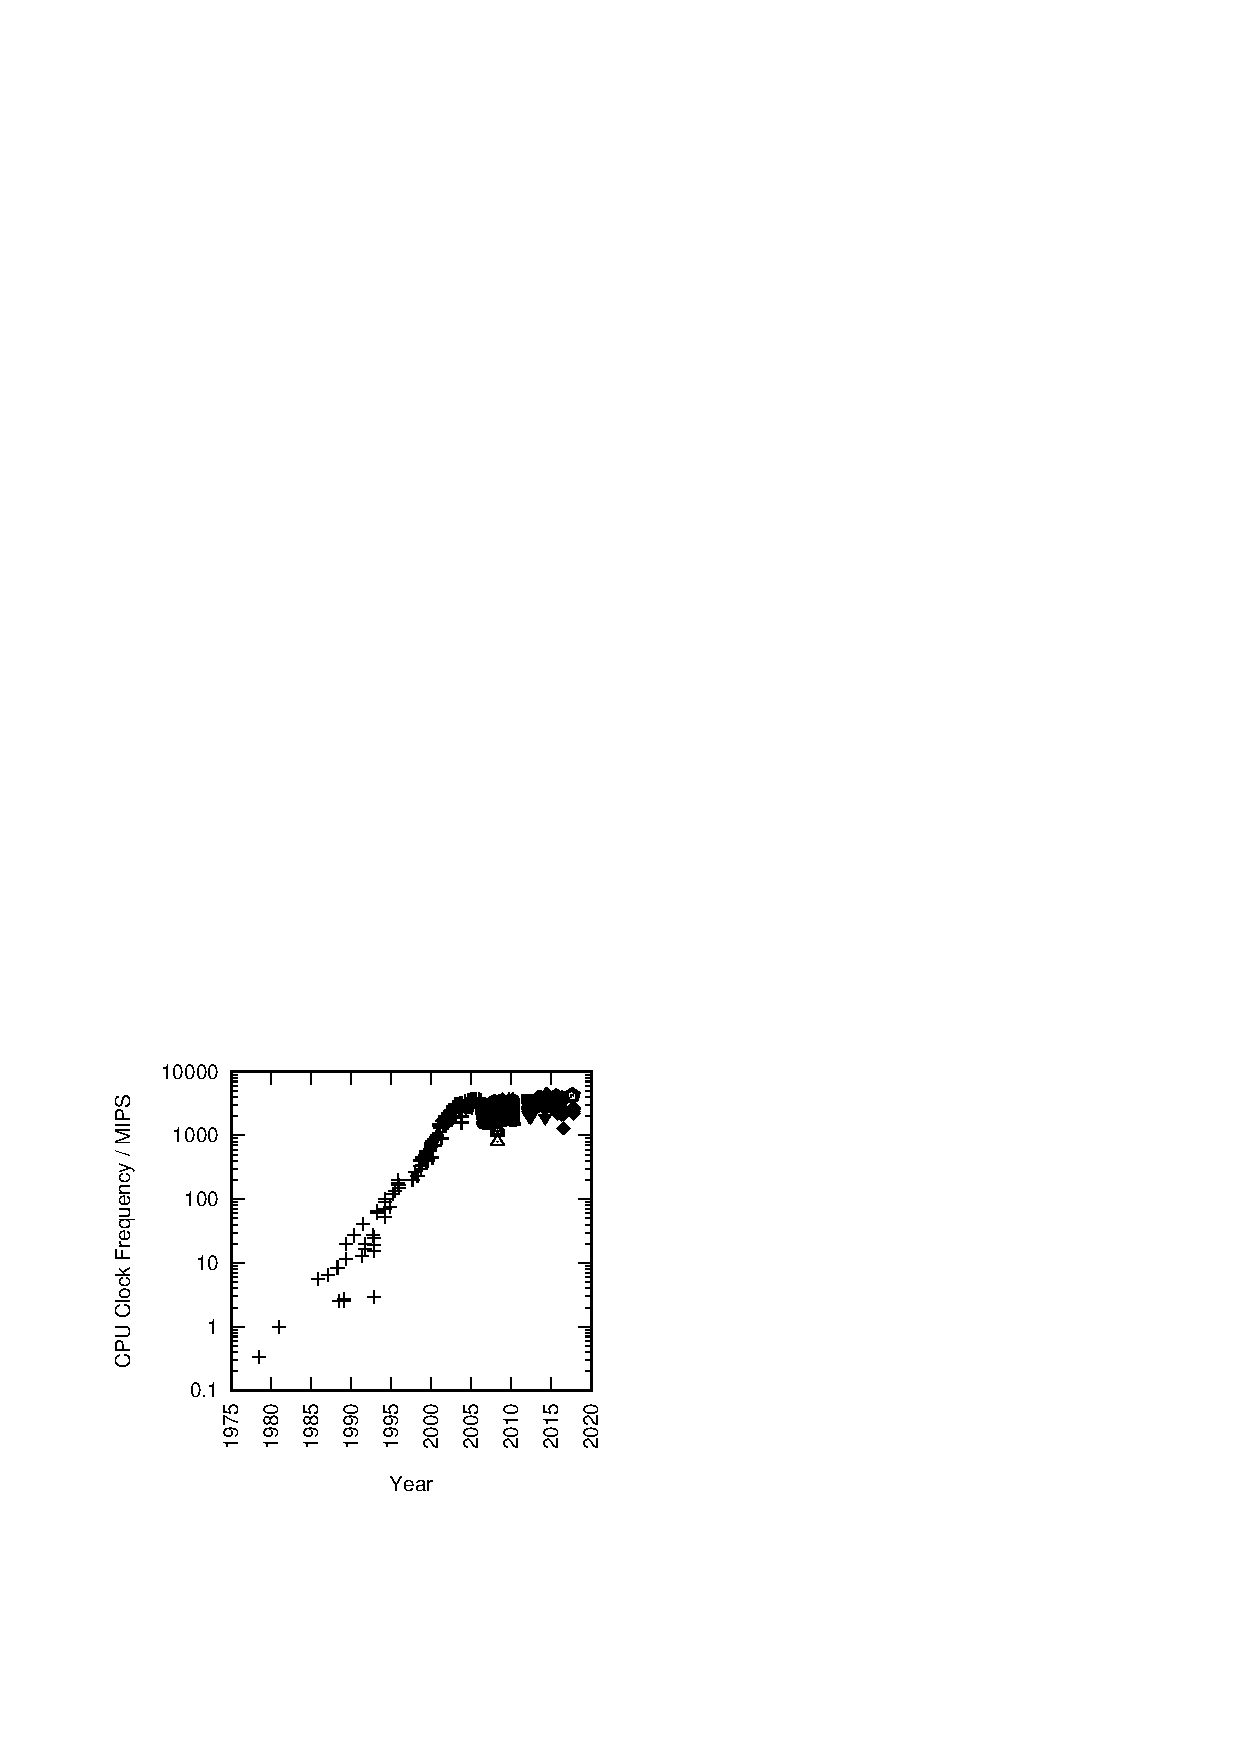
\includegraphics{SMPdesign/clockfreq}}
\end{center}
\caption{MIPS/Clock-Frequency Trend for Intel CPUs}
\label{fig:intro:Clock-Frequency Trend for Intel CPUs}
\end{figure}

그건 그렇고, 성능의 포커스는 하드웨어에서 병렬 소프트웨어로 옮겨졌습니다.
이는 무어의 법칙은 여전히 트랜지스터 밀집도를 높이고 있지만, 이를 전통적인
싱글쓰레드 성능 향상에 사용하는 것을 그만뒀기 때문이지요.
Figure~\ref{fig:intro:Clock-Frequency Trend for Intel CPUs} \footnote{
	이 그림은 이론상으로 한 클락에 한개 이상의 명령어를 처리할 수 있는 최신
	CPU 에서는 클락 주파수를, 그리고 가장 간단한 명령어의 처리에도 여러
	클락이 필요한 구형 CPU에서는 MIPS(오래된 Dhrystone 벤치마크에서 주로
	사용하던, millions of instructions per second) 를 보여줍니다.
	이렇게 서로 다른 두개의 측정 결과를 보여주는 이유는, 최신 CPU 의 한
	클락에 여러 명령어를 처리할 수 있는 기능이 일반적으로는 메모리쪽 성능에
	의해 제한되기 때문입니다.
	뿐만아니라, 구형 CPU 에서 일반적으로 사용되던 벤치마크는 너무 구식이고,
	최신의 벤치마크들을 구형 CPU 에서 돌리는건 구형 CPU를 구하기도 어려워서
	불가능에 가깝기 때문입니다.}
은 싱글쓰레드로 도는 코드를 작성하고 단순히 성능 목표를 만족할 더 빠른 컴퓨터가
나오길 1, 2 년 정도 기다리는건 더이상 선택지가 아니란 걸 보여줍니다.
모든 주요 제조사가 멀티코어/멀티쓰레드 시스템으로 개발 방향을 바꾼 이상,
병렬성만이 그런 시스템의 최대 성능을 끌어낼 수 있는 방법입니다.

\iffalse
That said, the focus of performance has shifted from hardware to
parallel software.
This change in focus is due to the fact that, although Moore's Law
continues to deliver increases in transistor density, it has ceased to
provide the traditional single-threaded performance increases.
This can be seen in
Figure~\ref{fig:intro:Clock-Frequency Trend for Intel CPUs}\footnote{
	This plot shows clock frequencies for newer CPUs theoretically
	capable of retiring one or more instructions per clock, and MIPS
	(millions of instructions per second, usually from the old
	Dhrystone benchmark)
	for older CPUs requiring multiple clocks to execute even the
	simplest instruction.
	The reason for shifting between these two measures is that the
	newer CPUs' ability to retire multiple instructions per clock is
	typically limited by memory-system performance.
	Furthermore, the benchmarks commonly used on the older CPUs
	are obsolete, and it is difficult to run the newer benchmarks
	on systems containing the old CPUs, in part because it is hard
	to find working instances of the old CPUs.},
which shows that writing single-threaded code and simply waiting
a year or two for the CPUs to catch up may no longer be an option.
Given the recent trends on the part of all major manufacturers towards
multicore/multithreaded systems, parallelism is the way to go for
those wanting the avail themselves of the full performance of their
systems.
\fi

하지만, 첫번째 목표는 성능이지 확장성이 아닙니다. 선형적인 확장성을 얻을 수
있는 가장 쉬운 방법이 각 CPU 의 성능을 떨어뜨리는
것~\cite{LinusTorvalds2001a}이기도 하고 말이죠.
네개 CPU 를 갖는 시스템을 갖게 되었다면, 당신은 뭘 고르시겠어요?
한개 CPU 위에서 초당 100개 트랜잭션을 처리하지만 CPU 확장성이 아예 없는
프로그램?
아니면 한개 CPU 위에선 초당 10개 트랜잭션만 처리하지만 완벽하게 CPU 를 늘려줌에
따라 성능이 늘어나는 프로그램?
아마 첫번째 프로그램이 더 나은 선택 같아 보이겠지만, 당신에게 32개 CPU 시스템이
생길 수 있다고 하면 또 답이 달라질겁니다.

\iffalse
Even so, the first goal is performance rather than scalability,
especially given that the easiest way to attain linear scalability
is to reduce the performance of each CPU~\cite{LinusTorvalds2001a}.
Given a four-CPU system, which would you prefer?
A program that provides 100 transactions per second on a single CPU,
but does not scale at all?
Or a program that provides 10 transactions per second on a single CPU,
but scales perfectly?
The first program seems like a better bet, though the answer might
change if you happened to have a 32-CPU system.
\fi

그렇다곤 하지만, 단순히 멀티 CPU 머신이 있기 때문이란 게 그 모든 CPU 를 다
사용해야 한다는 이유가 되진 않습니다. 특히나 요즘은 멀티 CPU 시스템이 매우 싼
가격이기도 하니까요.
이해해야 하는 핵심 포인트는 병렬 프로그래밍은 기본적으로 성능 최적화를 위한
여러 방법 중 하나란 거죠.
당신의 프로그램이 지금도 충분히 빠르다면 프로그램을 병렬화 시키거나 병렬화
이외의 다른 방법들을 통해 최적화를 할 필요 자체도 없습니다.\footnote{
	물론, 당신이 그저 취미로 병렬 소프트웨어를 만드는 사람이라면야
	그것만으로도 그 소프트웨어가 뭐건 병렬화를 할 충분한 이유가 되지요.}
같은 이유로, 당신이 최적화를 위해 시퀀셜 프로그램에 병렬성을 도입하려 한다면,
병렬 알고리즘들을 최선의 시퀀셜 알고리즘과 비교해야 합니다.
많은 병렬 알고리즘 성능 분석 문서들이 시퀀셜 알고리즘의 케이스를 아예
무시하고 있기 때문에 주의를 해야겠지만요.

\iffalse
That said, just because you have multiple CPUs is not necessarily
in and of itself a reason to use them all, especially given the
recent decreases in price of multi-CPU systems.
The key point to understand is that parallel programming is primarily
a performance optimization, and, as such, it is one potential optimization
of many.
If your program is fast enough as currently written, there is no
reason to optimize, either by parallelizing it or by applying any
of a number of potential sequential optimizations.\footnote{
	Of course, if you are a hobbyist whose primary interest is
	writing parallel software, that is more than enough reason to
	parallelize whatever software you are interested in.}
By the same token, if you are looking to apply parallelism as an
optimization to a sequential program, then you will need to compare
parallel algorithms to the best sequential algorithms.
This may require some care, as far too many publications ignore the
sequential case when analyzing the performance of parallel algorithms.
\fi

\subsection{Productivity}
\label{sec:intro:Productivity}

\QuickQuiz{}
	왜 이런 비기술적인 문제를 이야기하는거죠???
	그저 비기술적일 뿐 아니라, 심지어 \emph{생산성}이라니요?
	누가 그런걸 신경써요?

\iffalse
	Why all this prattling on about non-technical issues???
	And not just \emph{any} non-technical issue, but \emph{productivity}
	of all things?
	Who cares?
\fi
\QuickQuizAnswer{
	당신이 순수히 취미로만 사는 사람이라면 아마 당신은 신경쓰지 않아도
	될겁니다.
	하지만 설령 그렇다 해도 얼마나 빨리 그리고 얼마나 많이 일을 할 수
	있는지는 신경쓸겁니다.
	무엇보다, 가장 유명한 취미가용 도구는 보통 그 목적에 가장 적합한
	도구이고, ``가장 적합한'' 이란 말의 정의의 가장 중요한 부분은 생산성과
	연결되어 있죠.
	그리고 만약 누군가가 당신에게 병렬 코드를 작성하라고 돈을 준다면,
	그들은 당신의 생산성에 대해 매우 신경쓸겁니다.
	그리고 그 고용주가 뭔가에 신경쓴다면, 당신은 거기에 적어도 관심을
	가져야겠죠!

\iffalse
	If you are a pure hobbyist, perhaps you don't need to care.
	But even pure hobbyists will often care about how much they
	can get done, and how quickly.
	After all, the most popular hobbyist tools are usually those
	that are the best suited for the job, and an important part of
	the definition of ``best suited'' involves productivity.
	And if someone is paying you to write parallel code, they will
	very likely care deeply about your productivity.
	And if the person paying you cares about something, you would
	be most wise to pay at least some attention to it!
\fi

	그리고, 만약 당신이 \emph{정말로} 생산성에 신경쓰지 않는다면, 애초에
	컴퓨터를 사용하지 않고 손으로 일을 했겠죠!

\iffalse
	Besides, if you \emph{really} didn't care about productivity,
	you would be doing it by hand rather than using a computer!
\fi
} \QuickQuizEnd

최근 수십년간 생산성은 매우 중요해졌습니다.
엔지니어들의 연봉은 수천달러 정도인데 컴퓨터의 가격은 수천만 달러였던 과거를
생각해봅시다.
그당시의 컴퓨터에 10명의 엔지니어로 구성된 팀을 만들어서 성능을 10\% 라도
개선할 수 있다면, 그들은 많은 보너스를 받을 수 있었을겁니다.

\iffalse
Productivity has been becoming increasingly important in recent decades.
To see this, consider that the price of early computers was tens
of millions of dollars at
a time when engineering salaries were but a few thousand dollars a year.
If dedicating a team of ten engineers to such a machine would improve
its performance, even by only 10\%, then their salaries
would be repaid many times over.
\fi

CSIRAC 는 그런 부류의 머신 중 하나로, 가장 오래되었지만 여전히 온전한,
stored-program 컴퓨터로
1949년~\cite{CSIRACMuseumVictoria,CSIRACUniversityMelbourne}에 운영되었습니다.
이 머신은 트랜지스터 시대 이전에 만들어졌기 때문에, 2,000 개의 진공관으로
구성되었고 1kHz 클락 주파수로 동작했으며, 30kW 의 전력을 사용하고, 그 무게는
3톤이 넘었습니다.
하지만 이 머신은 768 워드밖에 안되는 용량의 RAM을 가지고 있었기에, 오늘날의
거대한 소프트웨어 프로젝트에서 종종 골치를 앓는 생산성 문제에서 자유로웠습니다.

\iffalse
One such machine was the CSIRAC, the oldest still-intact stored-program
computer, which was put into operation in
1949~\cite{CSIRACMuseumVictoria,CSIRACUniversityMelbourne}.
Because this machine was built before the transistor era, it was constructed
of 2,000 vacuum tubes, ran with a clock frequency of 1kHz,
consumed 30kW of power, and weighed more than three metric tons.
Given that this machine had but 768 words of RAM, it is safe to say that
it did not suffer from the productivity issues that often plague
today's large-scale software projects.
\fi

오늘날에 그렇게 성능이 떨어지는 기계를 구입하는건 매우 어렵습니다.
그나마 가장 비슷한 예는 Z80~\cite{z80Wikipedia}과 같은 8-bit 임베디드
마이크로프로세서가 될 수 있을 것 같습니다만, 그 Z80 조차도 CSIRAC 보다 1,000
배는 빠른 CPU 클락 주파수를 가지고 있었습니다.
Z80 CPU 는 8,500 개의 트랜지스터를 사용했고, 2008년도에 개당 \$2 US 에 1,000개
단위로 구매할 수 있었습니다.
CSIRAC 와 반대로 Z80 에서 소프트웨어 개발 비용은 그렇게 크게 중요하지
않았습니다.

\iffalse
Today, it would be quite difficult to purchase a machine with so
little computing power.
Perhaps the closest equivalents
are 8-bit embedded microprocessors exemplified by the venerable
Z80~\cite{z80Wikipedia}, but even the old Z80 had a CPU clock
frequency more than 1,000 times faster than the CSIRAC.
The Z80 CPU had 8,500 transistors, and could be purchased in 2008
for less than \$2 US per unit in 1,000-unit quantities.
In stark contrast to the CSIRAC, software-development costs are
anything but insignificant for the Z80.
\fi

\begin{figure}[tb]
\begin{center}
\resizebox{3in}{!}{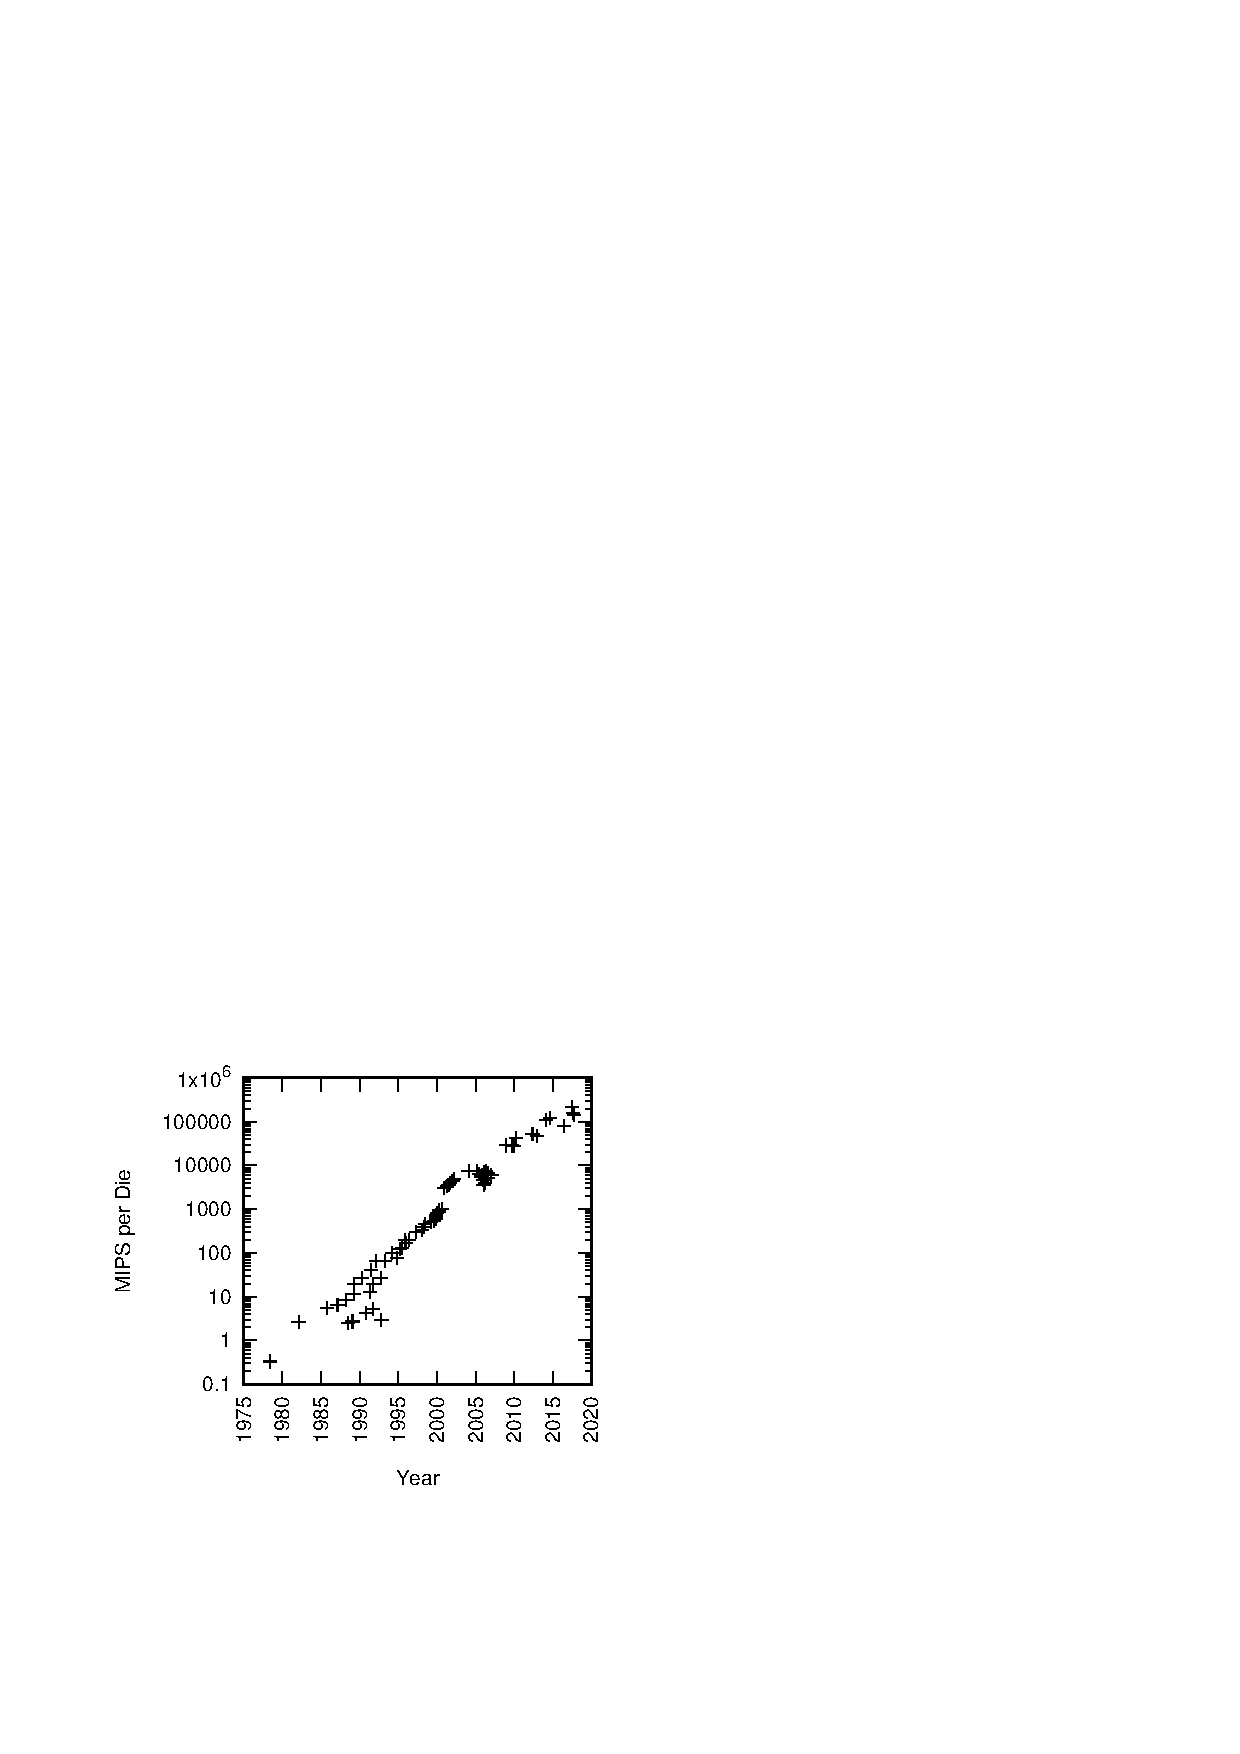
\includegraphics{SMPdesign/mipsperbuck}}
\end{center}
\caption{MIPS per Die for Intel CPUs}
\label{fig:intro:MIPS per Die for Intel CPUs}
\end{figure}

오랫동안의 트렌드를 Figure~\ref{fig:intro:MIPS per Die for Intel CPUs} 를 통해
보면 CSIRAC 와 Z80 은 그 가운데 두개의 점으로 표현될 수 있습니다.
이 그림은 지난 30여년간의 다이당 컴퓨테이션 파워 변화를 간략히 보여주는데,
지속적으로 증가한 걸 볼 수 있습니다.
멀티코어 CPU 의 성장은 2003년에 마주한 클락 주파수의 한계 장벽에도 불과하고
이런 증가 추세를 지속시켰습니다.

\iffalse
The CSIRAC and the Z80 are two points in a long-term trend, as can be
seen in
Figure~\ref{fig:intro:MIPS per Die for Intel CPUs}.
This figure plots an approximation to computational power per die
over the past three decades, showing a consistent four-order-of-magnitude
increase.
Note that the advent of multicore CPUs has permitted this increase to
continue unabated despite the clock-frequency wall encountered in 2003.
\fi

이렇게 가파른 하드웨어 가격 하락은 소프트웨어 생산성이 점점 중요해짐을 의미합니다.
이제는 그저 하드웨어를 효과적으로 사용하는 것만으로는 충분하지 않습니다:
이젠 소프트웨어 개발자들을 가능한한 효과적으로 사용하는 것이 중요합니다.
시퀀셜 하드웨어에서는 예전부터 그런 문제가 있었지만, 병렬 하드웨어는 최근에서야
낮은 가격으로 상품이 나오기 시작했습니다.
따라서, 병렬 소프트웨어를 만들때의 생산성은 최근에 들어서야 매우
중요해졌습니다.

\iffalse
One of the inescapable consequences of the rapid decrease in
the cost of hardware is that software productivity becomes increasingly
important.
It is no longer sufficient merely to make efficient use of the hardware:
It is now necessary to make extremely efficient use of software
developers as well.
This has long been the case for sequential hardware, but
parallel hardware has become a low-cost commodity only recently.
Therefore, only recently has high productivity become critically important
when creating parallel software.
\fi

\QuickQuiz{}
	병렬 시스템이 그렇게 싼 가격이 되었다면, 어떤 사람이 그걸 프로그램
	하라고 월급을 줘가며 프로그래머를 고용하겠어요?
\iffalse
	Given how cheap parallel systems have become, how can anyone
	afford to pay people to program them?
\fi
\QuickQuizAnswer{
	이 질문에는 몇가지 답이 있습니다:
	\begin{enumerate}
	\item	거대한, 여러 병렬머신들로 구성된 클러스터가 있다고 하면, 이 클러스터의 전체 비용은 상당한 개발 노력을 정당화합니다. 개발 비용은 수많은 머신들 전체에게 적용되기 때문이죠.
	\item	수천만명이 넘는 사용자들이 사용하는 유명한 소프트웨어라면 상당한 개발 노력이 정당화 됩니다. 그 개발 노력은 수천만 사용자를 위한 거니까요.
		커널이나 시스템 라이브러리 같은 것들도 이 경우에 들어감을 참고하세요.
	\item	낮은 가격의 병렬 머신이 중요한 어떤 장비의 운영에 사용되고 있다면 그 장비의 가격 일부분이 상당한 개발 비용을 정당화 할 수 있습니다.
	\item	안전을 위해 사용되는 주요 시스템은 사람의 목숨을 보호합니다. 따라서 이 경우에는 매우 큰 개발 비용을 정당화 하죠.
	\item	취미가와 연구자들은 돈보다는 지식, 경험, 재미, 그리고 명예를 추구합니다.
	\end{enumerate}
	그러니까 하락하는 하드웨어 가격은 소프트웨어를 의미없게 만들지 않고,
	오히려 소프트웨어 개발 비용을 하드웨어 가격에 ``숨기는'' 것이
	불가능해진 겁니다. 적어도 엄청나게 많은 수의 하드웨어를 사용하는 경우가
	아니라면요.

\iffalse
	There are a number of answers to this question:
	\begin{enumerate}
	\item	Given a large computational cluster of parallel machines,
		the aggregate cost of the cluster can easily justify
		substantial developer effort, because the development
		cost can be spread over the large number of machines.
	\item	Popular software that is run by tens of millions of users
		can easily justify substantial developer effort,
		as the cost of this development can be spread over the tens
		of millions of users.
		Note that this includes things like kernels and system
		libraries.
	\item	If the low-cost parallel machine is controlling the operation
		of a valuable piece of equipment, then the cost of this
		piece of equipment might easily justify substantial
		developer effort.
	\item	If the software for the low-cost parallel machine produces an
		extremely valuable result (e.g., mineral exploration),
		then the valuable result might again justify substantial
		developer cost.
	\item	Safety-critical systems protect lives, which can clearly
		justify very large developer effort.
	\item	Hobbyists and researchers might seek knowledge, experience,
		fun, or glory rather than gold.
	\end{enumerate}
	So it is not the case that the decreasing cost of hardware renders
	software worthless, but rather that it is no longer possible to
	``hide'' the cost of software development within the cost of
	the hardware, at least not unless there are extremely large
	quantities of hardware.
\fi
} \QuickQuizEnd

적어도 한때에는 병렬 소프트웨어의 유일한 목표가 성능이었습니다. 하지만, 지금은
생산성이 점점 스포트라이트를 받고 있습니다.

\iffalse
Perhaps at one time, the sole purpose of parallel software was performance.
Now, however, productivity is gaining the spotlight.
\fi

\subsection{Generality}
\label{sec:intro:Generality}

병렬 소프트웨어를 개발하는 높은 비용을 정당화 할 수 있는 한가지 방법은 최대한의
generality 를 위해 노력하는 것입니다.
보다 일반적인 소프트웨어 제품의 개발 비용은 덜 일반적인 것에 비해 더 많은
사용자들로 나뉘어져 보상되기 때문입니다.
실제로, 이런 경제적 이유가 generality 의 중요한 특별 케이스라 할 수 있는
이식성에 대한 마니악한 관심을 설명합니다.\footnote{
	이걸 지적해준 Michael Wong 에게 찬사를.}

\iffalse
One way to justify the high cost of developing parallel software
is to strive for maximal generality.
All else being equal, the cost of a more-general software artifact
can be spread over more users than that of a less-general one.
In fact, this economic force explains much of the maniacal focus
on portability, which can be seen as an important special case
of generality.\footnote{
	Kudos to Michael Wong for pointing this out.}
\fi

불행히도, generality 는 종종 성능이나 생산성, 또는 둘 다를 하락시키기도 합니다.
예를 들어, 이식성은 종종 중간 레이어를 두는 식으로 만족되는데, 중간 레이어가
추가되는 것은 분명한 성능 하락을 야기합니다.
보다 일반적인 환경에서의 이 현상을 보기 위해, 다음의 널리 쓰이는 병렬
프로그래밍 환경들을 생각해봅시다:

\iffalse
Unfortunately, generality often comes at the cost of performance,
productivity, or both.
For example, portability is often achieved via adaptation layers,
which inevitably exact a performance penalty.
To see this more generally, consider the following popular parallel
programming environments:
\fi

\begin{description}
\item[C/C++ ``락킹과 쓰레드'']: POSIX
	쓰레드(pthreads)~\cite{OpenGroup1997pthreads}, Windows 쓰레드, 그리고
	많은 운영체제 커널 환경을 포함하는 이 카테고리는 (최소 하나의 SMP
	시스템에서는) 엄청난 성능과 좋은 generality 를 제공합니다.
	비교적 낮은 생산성은 아쉽지만요.

\iffalse
\item[C/C++ ``Locking Plus Threads'']: This category, which includes
	POSIX Threads (pthreads)~\cite{OpenGroup1997pthreads},
	Windows Threads, and numerous
	operating-system kernel environments, offers excellent performance
	(at least within the confines of a single SMP system)
	and also offers good generality.
	Pity about the relatively low productivity.
\fi

\item[Java]: 이 범용적이고 본질적으로 멀티쓰레드를 고려한 프로그래밍 환경은
	자동 가비지 콜렉터와 당야한 클래스 라이브러리들로 인해 C 나 C++ 보다
	훨씬 높은 생산성을 제공하는 것으로 널리 알려졌습니다.
	하지만, 그 성능은 2000년대 초에 엄청 개선되긴 했지만 여전히 C 와 C++
	보다 부족합니다.

\iffalse
\item[Java]: This general purpose and inherently multithreaded
	programming environment	is widely believed to offer much higher
	productivity than C or C++, courtesy of the automatic garbage collector
	and the rich set of class libraries.
	However, its performance, though greatly improved in the early
	2000s, lags that of C and C++.
\fi

\item[MPI]: 이 메세지 패싱 인터페이스~\cite{MPIForum2008} 는 세계에서 가장 큰
	과학 분야와 기술 분야 컴퓨팅 클러스터들을 뒷받침하며 병렬화 되지 않은
	성능과 확장성을 제공합니다.
	그러나, 이론적으로는 범용적으로 사용 가능하다고 하지만 대부분의 경우
	과학 분야와 기술 분야 컴퓨팅에서 사용됩니다.
	그 생산성은 심지어 C/C++ ``락킹과 쓰레드'' 환경보다도 떨어진다고 많은
	사람들이 생각합니다.

\iffalse
\item[MPI]: This Message Passing Interface~\cite{MPIForum2008} powers
	the largest scientific and technical computing clusters in
	the world and offers unparalleled performance and scalability.
	In theory, it is general purpose, but it is mainly used
	for scientific and technical computing.
	Its productivity is believed by many to be even lower than that
	of C/C++ ``locking plus threads'' environments.
\fi

\item[OpenMP]: 이 컴파일러 지시어 집합은 루프문을 병렬화 하는데 사용될 수
	있습니다.
	때문에 이 특정한 작업에 한정적이고, 이런 제약이 종종 그 성능을
	제한합니다.
	하지만, MPI 나 C/C++ ``락킹과 쓰레드'' 보다는 사용하기 쉬운 편입니다.

\iffalse
\item[OpenMP]: This set of compiler directives can be used
	to parallelize loops.  It is thus quite specific to this
	task, and this specificity often limits its performance.
	It is, however, much easier to use than MPI or C/C++
	``locking plus threads.''
\fi

\item[SQL]: SQL (Structured Query Language~\cite{DIS9075SQL92} 는 관계형
	데이터베이스 쿼리에 제한적입니다.
	하지만, 그 성능은 트랜잭션 처리 성능 의회 (TPC) 벤치마크
	결과들~\cite{TPC}로 볼 때 상당히 좋습니다.
	생산성도 대단합니다; 실제로, 이 병렬 프로그래밍 환경은 병렬 프로그래밍
	컨셉을 잘 모르거나 아예 모르는 사람들도 커다란 병렬 시스템을 잘 사용할
	수 있게 돕습니다.

\iffalse
\item[SQL]: Structured Query Language~\cite{DIS9075SQL92} is
	specific to relational database queries.
	However, its performance is quite good as measured by the
	Transaction Processing Performance Council (TPC)
	benchmark results~\cite{TPC}.
	Productivity is excellent; in fact, this parallel programming
	environment enables people to make good use of a large parallel
	system despite having little or no knowledge of parallel
	programming concepts.
\fi
\end{description}

\begin{figure}[tb]
\begin{center}
\resizebox{3in}{!}{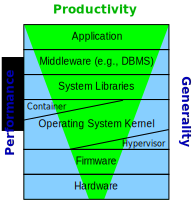
\includegraphics{intro/PPGrelation}}
\end{center}
\caption{Software Layers and Performance, Productivity, and Generality}
\label{fig:intro:Software Layers and Performance, Productivity, and Generality}
\end{figure}

훌륭한 성능, 생산성, 그리고 generality 를 제공하는 병렬 프로그래밍 환경의
천국은 아직 존재하지 않습니다.
그런 천국이 오기 전까지는, 성능, 생산성, 그리고 generality 사이에서
엔지니어링적 트레이드오프를 가질 수밖에 없습니다.
그런 트레이드오프의 한 예가 Figure~\ref{fig:intro:Software Layers and
Performance, Productivity, and Generality} 에 있습니다; 이 그림은 시스템 스택의
상위 레이어로 갈수록 생산성은 점점 중요해지고 성능과 generality 는 하위
레이어로 갈수록 중요해진다는 점을 보여줍니다.
하위 레이어에서 발생하는 거대한 개발 비용은 똑같이 거대한 사용자 수로
나뉘어져야 하고(그래서 generality 가 중요하죠), 하위 레이어에서 잃은 성능은
위쪽에서 쉽게 회복시킬 수 없습니다. 
스택의 윗단에서는 해당 특정 어플리케이션에 대해 매우 적은 사용자만
존재할겁니다. 생산성 고려가 중요해지죠.
이게 스택의 위로 갈수록 ``bloatware''가 되는 경향을 설명합니다:
많은 경우 여분의 하드웨어가 여분의 개발자보다 싸게 먹히니까요.
이 책은 성능과 generality 가 주요 관심사인, 스택의 바닥 근처에 있는 개발자를
대상으로 합니다.

\iffalse
The nirvana of parallel programming environments, one that offers
world-class performance, productivity, and generality, simply does
not yet exist.
Until such a nirvana appears, it will be necessary to make engineering
tradeoffs among performance, productivity, and generality.
One such tradeoff is shown in
Figure~\ref{fig:intro:Software Layers and Performance, Productivity, and Generality},
which shows how productivity becomes increasingly important at the upper layers
of the system stack,
while performance and generality become increasingly important at the
lower layers of the system stack.
The huge development costs incurred at the lower layers
must be spread over equally huge numbers of users
(hence the importance of generality), and
performance lost in lower layers cannot easily be
recovered further up the stack.
In the upper layers of the stack, there might be very few users for a given
specific application, in which case productivity concerns are paramount.
This explains the tendency towards ``bloatware'' further up the stack:
extra hardware is often cheaper than the extra developers.
This book is intended for developers working near the bottom
of the stack, where performance and generality are of great concern.
\fi

\begin{figure}[tb]
\begin{center}
\resizebox{3in}{!}{\includegraphics{intro/Generality}}
\end{center}
\caption{Tradeoff Between Productivity and Generality}
\label{fig:intro:Tradeoff Between Productivity and Generality}
\end{figure}

생산성과 generality 사이에서의 트레이드오프가 많은 영역에서 100여년간
존재했음을 알아둘 필요가 있습니다.
하나만 예를 들자면, 못을 박는데 망치보다 레일건이 생산적이지만 망치는 못박는 거
말고도 많은 영역에 사용될 수 있죠.
그러니 병렬 컴퓨팅에서도 비슷한 트레이드오프들을 발견하는건 그다지 놀라운 일이
아닙니다.
이런 트레이드오프는 추상적으로 Figure~\ref{fig:intro:Tradeoff Between
Productivity and Generality} 에 나타나 있습니다.
여기서 user~1, 2, 3, 그리고 4 는 컴퓨터가 도와야 하는 그들만의 특정한 작업을
가지고 있습니다.
특정 사용자에게 가장 생산적인 언어 또는 환경은 어떤 프로그래밍이나 환경 설정,
환경 구축을 할 필요 없이 간단하게 그 사용자의 작업을 해내는 언어 또는
환경입니다.

\iffalse
It is important to note that a tradeoff between productivity and
generality has existed for centuries in many fields.
For but one example, a nailgun is more productive than a hammer for
driving nails, but in contrast to the nailgun, a hammer can be used for
many things besides driving nails.
It should therefore be no surprise to see similar tradeoffs
appear in the field of parallel computing.
This tradeoff is shown schematically in
Figure~\ref{fig:intro:Tradeoff Between Productivity and Generality}.
Here, users~1, 2, 3, and 4 have specific jobs that they need the computer
to help them with.
The most productive possible language or environment for a given user is one
that simply does that user's job, without requiring any programming,
configuration, or other setup.
\fi

\QuickQuiz{}
	이건 달성 불가한 이상에 불과해요!
	현실적으로 달성 가능한 무언가에 집중하는게 어때요?

\iffalse
	This is a ridiculously unachievable ideal!
	Why not focus on something that is achievable in practice?
\fi
\QuickQuizAnswer{
	이건 분명 달성 가능합니다.
	휴대폰은 프로그래밍이나 환경구성 없이 최종 사용자가 전화 통화를 하고
	텍스트 메세지를 주고 받을 수 있게 해주는 컴퓨터입니다.

\iffalse
	This is eminently achievable.
	The cellphone is a computer that can be used to make phone
	calls and to send and receive text messages with little or
	no programming or configuration on the part of the end user.
\fi

	일견 사소한 예처럼 보일 수 있겠지만, 천천히 생각해보면 이건 간단하기도
	하고 심오하기도 한 이야기입니다.
	generality 를 희생하면 우리는 놀랍도록 높은 생산성 향상을 얻을 수
	있습니다.
	과한 generality 에 빠진 사람들은 그래서 소프트웨어 스택의 최대치까지
	성능을 끌어올리는데 실패하곤 합니다.
	이 삶의 진리는 약자도 있죠: YAGNI, 즉 ``You Ain't Gonna Need It.''

\iffalse
	This might seem to be a trivial example at first glance,
	but if you consider it carefully you will see that it is
	both simple and profound.
	When we are willing to sacrifice generality, we can achieve
	truly astounding increases in productivity.
	Those who indulge in excessive generality will therefore fail to set
	the productivity bar high enough to succeed near the top of the
	software stack.
	This fact of life even has its own acronym: YAGNI, or ``You
	Ain't Gonna Need It.''
\fi
} \QuickQuizEnd

불행히도, user~1 에 의해 요청된 작업을 수행하는 시스템은 user~2 의 작업을
처리하지 못하는 경우가 많습니다.
가장 생산성 좋은 언어와 환경은 영역이 한정되어 있어서, generality 가 부족할 수
있다는 것이죠.

\iffalse
Unfortunately, a system that does the job required by user~1 is
unlikely to do user~2's job.
In other words, the most productive languages and environments are
domain-specific, and thus by definition lacking generality.
\fi

다른 선택지는 Figure~\ref{fig:intro:Tradeoff Between Productivity and
Generality} 의 가운데 영역처럼 프로그래밍 언어나 환경을 주어진 (assembly, C,
C++, 또는 Java 같은 로우 레벨 언어들처럼) 하드웨어나 (Haskell, Prolog, 또는
Snobol 처럼) 추상화에 맞추는 것입니다.
이런 언어들은 user~1, 2, 3, 4 에 의해 요청된 작업들에 대해 모두 똑같이 맞춰져
있지 않다는 점에서 일반적이라고 할 수 있습니다.
다시 말해, 그런 언어들의 generality 는 해당 영역에 한정된 언어와 환경에 비해
생산성을 떨어뜨려야만 얻을 수 있다는 거죠.
뿐만 아니라, 특정 추상화에 맞춰진 언어는 누군가가 그 추상화와 실제 하드웨어
사이의 매핑을 효과적으로 하기 전까지는 성능과 확장성 문제를 심하게 겪을 확률이
높습니다.

\iffalse
Another option is to tailor a given programming language or environment
to the hardware system (for example, low-level languages such as
assembly, C, C++, or Java) or to some abstraction (for example,
Haskell, Prolog, or Snobol), as is shown by the circular region near
the center of
Figure~\ref{fig:intro:Tradeoff Between Productivity and Generality}.
These languages can be considered to be general in the sense that they
are equally ill-suited to the jobs required by users~1, 2, 3, and 4.
In other words, their generality is purchased at the expense of
decreased productivity when compared to domain-specific languages
and environments.
Worse yet, a language that is tailored to a given abstraction
is also likely to suffer from performance and scalability problems
unless and until someone figures out how to efficiently map that
abstraction to real hardware.
\fi

성능, 생산성, generality 라는 쇠로된 삼각형의 세가지 목표에서의 탈출은 불가능한
걸까요?

\iffalse
Is there no escape from iron triangle's three conflicting goals of
performance, productivity, and generality?
\fi

실은 종종 탈출구가 있습니다. 예를 들어, 다음 섹션에서 이야기할 병렬
프로그래밍의 대안책을 사용하는 것이죠.
병렬 프로그래밍은 엄청난 재미를 가져다 줄 수는 있지만, 항상 최고의 선택인 건
아닙니다.

\iffalse
It turns out that there often is an escape, for example,
using the alternatives to parallel programming discussed in the next section.
After all, parallel programming can be a great deal of fun, but
it is not always the best tool for the job.
\fi

\section{Alternatives to Parallel Programming}
\label{sec:intro:Alternatives to Parallel Programming}

병렬 프로그래밍의 대안을 제대로 고려해보려면, 당신은 당신이 병렬성에 기대하는게
뭔지 정확히 정해야 합니다.
Section~\ref{sec:intro:Parallel Programming Goals} 에서 본것과 같이, 병렬
프로그래밍의 주요 목표는 성능, 생산성, 그리고 generality 입니다.
이 책은 소프트웨어 스택의 바닥 근처에서 성능에 큰 영향을 끼치는 코드를 만지는
개발자들을 대상으로 하고 있기 때문에, 이 섹션의 나머지 부분은 성능 개선 쪽에
포커스를 맞춥니다.

\iffalse
In order to properly consider alternatives to parallel programming,
you must first decide on what exactly you expect the parallelism
to do for you.
As seen in Section~\ref{sec:intro:Parallel Programming Goals},
the primary goals of parallel programming are performance, productivity,
and generality.
Because this book is intended for developers working on
performance-critical code near the bottom of the software stack,
the remainder of this section focuses primarily on performance improvement.
\fi

병렬성은 성능을 개선하기 위한 방법 중 하나에 불과하단 것을 명심해야 합니다.
병렬성 외의 잘 알려진 방법을 적당히 덜 어려운 순서에서 더 어려운 순서로 나열해
보자면 다음과 같습니다:

\iffalse
It is important to keep in mind that parallelism is but one way to
improve performance.
Other well-known approaches include the following, in roughly increasing
order of difficulty:
\fi

\begin{enumerate}
\item	시퀀셜 어플리케이션의 여러 인스턴스를 실행하는것.
\item	어플리케이션이 이미 존재하는 병렬 소프트웨어를 사용하게 하는것.
\item	성능 개선책을 시리얼 어플리케이션에 적용하는것.

\iffalse
\item	Run multiple instances of a sequential application.
\item	Make the application use existing parallel software.
\item	Apply performance optimization to the serial application.
\fi
\end{enumerate}

이 방법들 각각을 다음의 섹션들에서 설명합니다.

\iffalse
These approaches are covered in the following sections.
\fi

\subsection{Multiple Instances of a Sequential Application}
\label{sec:intro:Multiple Instances of a Sequential Application}

시퀀셜 어플리케이션의 인스턴스를 여러개 실행시키는 것으로 당신은 실제로는 병렬
프로그래밍을 하지 않으지만 병렬 프로그래밍을 한것과 같은 효과를 얻을 수
있습니다.
이런 접근법에는 어플리케이션의 구조에 따라 여러 방법이 있습니다.

\iffalse
Running multiple instances of a sequential application can allow you
to do parallel programming without actually doing parallel programming.
There are a large number of ways to approach this, depending on the
structure of the application.
\fi

당신의 프로그램이 매우 많은, 서로 다른 시나리오를 분석하거나 매우 많은 독립적
데이터 셋을 분석하는 것이라면 쉽고 효과적인 방법 하나는 하나의 분석을 수행하는
하나의 시퀀셜 프로그램을 만들고 (예를 들면 \co{bash} 셸 같은) 스크립트 환경을
사용해 그 시퀀셜 프로그램의 여러 인스턴스를 병렬적으로 수행시키는 것입니다.
경우에 따라서는 이런 접근법은 여러 머신으로 구성된 클러스터로도 쉽게 확장될 수
있습니다.

\iffalse
If your program is analyzing a large number of different scenarios,
or is analyzing a large number of independent data sets, one easy
and effective approach is to create a single sequential program that
carries out a single analysis, then use any of a number of scripting
environments (for example the \co{bash} shell) to run a number of
instances of that sequential program in parallel.
In some cases, this approach can be easily extended to a cluster of
machines.
\fi

이런 접근법은 사기처럼 보일수도 있겠죠, 그리고 어떤 사람들은 그런 프로그램들을
``당황 스러울 정도로 병렬적이다'' 라고 폄하합니다.
그리고 실제로, 이런 접근법은 증가된 메모리 소모, 같은 중간 결과를 다시
계산함으로써 발생하는 CPU 사이클의 낭비, 그리고 증가된 데이터 복사와 같은
잠재적 단점을 갖습니다.
하지만, 이 접근은 종종 매우 생산적이어서 엄청난 생산성 증가를 매우 적은, 또는
아예 없는 추가 노력으로도 달성 가능하게 해줍니다.

\iffalse
This approach may seem like cheating, and in fact some denigrate such
programs as ``embarrassingly parallel''.
And in fact, this approach does have some potential disadvantages,
including increased memory consumption, waste of CPU cycles recomputing
common intermediate results, and increased copying of data.
However, it is often  extremely productive, garnering extreme performance
gains with little or no added effort.
\fi

\subsection{Use Existing Parallel Software}
\label{sec:intro:Use Existing Parallel Software}

관계형 데이터베이스~\cite{Date82}, 웹 어플리케이션 서버, 그리고 맵 리듀스 환경
등과 같이 싱글 쓰레드 프로그래밍으로 동작시킬 수 있는 병렬 소프트웨어 환경이
오늘날에는 결코 적지 않습니다.
예를 들어, 흔한 구조 중 하나는 각자 SQL 프로그램을 생성하는 별개의 프로그램을
각 유저에게 제공하는 것입니다(역주: SQL 클라이언트 같은거죠).
이렇게 유저별로 배포된 SQL 프로그램은, 자동으로 사용자들의 쿼리를 동시에
처리하는 일반적인 관계형 데이터베이스와 상호 동작합니다.
사용자에게 배포된 프로그램은 단지 사용자 인터페이스만 책임지면 되고,
병렬성과 데이터 정합성 등의 어려운 일은 모두 관계형 데이터베이스의 책임입니다.

\iffalse
There is no longer any shortage of parallel software environments that
can present a single-threaded programming environment,
including relational
databases~\cite{Date82},
web-application servers, and map-reduce environments.
For example, a common design provides a separate program for each
user, each of which generates SQL programs.
These per-user SQL programs are run concurrently against a common
relational database, which automatically runs the users' queries concurrently.
The per-user programs are responsible only for the user interface,
with the relational database taking full responsibility for the
difficult issues surrounding parallelism and persistence.
\fi

또한, 특히 수학 계산 쪽에서, 병렬 라이브러리 함수들도 많이 생겨나고 있습니다.
심지어 일부 라이브러리는 벡터 연산 유닛들과 범용 그래픽 처리 유닛 (GPGPU)와
같은, 특정 목적으로 만들어진 하드웨어의 특성을 활용하기도 합니다.

\iffalse
In addition, there are a growing number of parallel library functions,
particularly for numeric computation.
Even better, some libraries take advantage of special-purpose
hardware such as vector units and general-purpose graphical processing
units (GPGPUs).
\fi

매우 신경써서 조심스럽게 만들어진 완전히 병렬적인 어플리케이션에 비교했을 때엔
이런 접근법은 종종 성능을 희생합니다.
하지만, 그정도 희생은 대부분의 경우 커다란 개발 비용의 축소로 보상됩니다.

\iffalse
Taking this approach often sacrifices some performance, at least when
compared to carefully hand-coding a fully parallel application.
However, such sacrifice is often well repaid by a huge reduction in
development effort.
\fi

\QuickQuiz{}
	잠깐만요!
	이런 접근법은 단순히 개발을 위한 노력을 당신으로부터 누군가 그
	존재한다는 병렬 소프트웨어를 만드는 사람에게 전가할 뿐인 거 아닌가요?
\iffalse
	Wait a minute!
	Doesn't this approach simply shift the development effort from
	you to whoever wrote the existing parallel software you are using?
\fi
\QuickQuizAnswer{
	바로 그겁니다!
	그리고 그게 바로 이미 있는 소프트웨어를 쓰는 것의 요점이죠.
	한 팀의 작업물이 많은 다른 팀에 의해 사용되어서 모든 팀이 불필요하게
	바퀴를 재발명하는 것에 비해 훨씬 노력을 줄이게 되는것이요.
\iffalse
	Exactly!
	And that is the whole point of using existing software.
	One team's work can be used by many other teams, resulting in a
	large decrease in overall effort compared to all teams
	needlessly reinventing the wheel.
\fi
} \QuickQuizEnd

\subsection{Performance Optimization}
\label{sec:intro:Performance Optimization}

2000년대 초까지, CPU 성능은 매 18개월마다 두배씩 빨라졌습니다.
그런 환경에서는 조심스럽게 성능을 개선하는 것보다 새로운 기능을 추가하는 것이
대부분의 경우 중요합니다.
무어의 법칙은 트랜지스터 집적도와 트랜지스터당 성능을 높이는 게 아니라,
``단지'' 트랜지스터 집적도만을 올리기 때문에 지금은 성능 최적화의 중요성에 대해
다시 생각해볼 좋은 기회입니다.
무엇보다, 새로운 하드웨어들은 더이상 대단한 싱글 쓰레드 성능 향상을 가져오지
않습니다.
더우기, 많은 성능 최적화는 에너지 소모를 줄입니다.

\iffalse
Up through the early 2000s, CPU performance was doubling every 18 months.
In such an environment, it is often much more important to create new
functionality than to do careful performance optimization.
Now that Moore's Law is ``only'' increasing transistor density instead
of increasing both transistor density and per-transistor performance,
it might be a good time to rethink the importance of performance
optimization.
After all, new hardware generations no longer bring significant
single-threaded performance improvements.
Furthermore, many performance optimizations can also conserve energy.
\fi

이런 관점에서, 병렬 시스템이 점점 싸고 시장에 많이 나올수록 더욱더 매력적인
성능 개선 방법이 되고 있습니다.
하지만, 병렬성을 활용해 얻을 수 있는 성능 향상 정도는 대략적으로 보면, CPU 수에
제한됨을 기억하고 있는게 현명할 것입니다.
반면, 전통적인 싱글 쓰레드 소프트웨어 최적화에서의 최적화 기법을 통한 성능
향상은 그보다 훨씬 클 수 있습니다.
예를 들어, 긴 링크드 리스트를 해쉬 테이블이나 서치 트리로 교체하는 것은
수십수백배 성능을 향상시킬 수 있습니다.
이 고도로 최적화된 싱글쓰레드 프로그램은 최적화 되지 않은 병렬 프로그램에 비해
훨씬 빠를 것이고, 병렬성은 필요치 않을 것입니다.
물론, 고도로 최적화된 병렬 프로그램은 추가적인 개발과정의 노력이 필요하겠지만
최적화된 싱글쓰레드 프로그램보다도 나은 성능을 보일테죠.

\iffalse
From this viewpoint, parallel programming is but another performance
optimization, albeit one that is becoming much more attractive
as parallel systems become cheaper and more readily available.
However, it is wise to keep in mind that the speedup available from
parallelism is limited to roughly the number of CPUs.
In contrast, the speedup available from traditional single-threaded
software optimizations can be much larger.
For example, replacing a long linked list with either a hash table
or a search tree can improve performance by many orders of magnitude.
This highly optimized single-threaded program might run much
faster than its unoptimized parallel counterpart, making parallelization
unnecessary.
Of course, a highly optimized parallel program would be even better,
give or take the added development effort required.
\fi

더욱이, 서로 다른 프로그램들은 서로 다른 성능 병목지점을 가질 겁니다.
예를 들어, 당신의 프로그램이 대부분의 시간을 디스크 드라이브로부터 읽어들이는
데이터가 도착하기를 기다리고 있다면, 여러 CPU 를 사용하는 것은 그저
디스크로부터 데이터를 기다리는 시간을 증가시키기만 할수도 있습니다.
실제로, 프로그램이 하드디스크처럼 회전하는 디스크에 시퀀셜하게 씌여져 있는
하나의 큰 파일을 읽으려 할 때, 그 프로그램을 병렬화 하면 추가된 탐색 오버헤드
때문에 프로그램이 더 느려질 수 있습니다.
그보다는 데이터 배치를 그 파일이 더 작아질 수 있도록 (그래서 더 빨리 읽어들일
수 있도록) 하고, 그 파일을 병렬적으로 다른 드라이브에서 접근할 수 있도록, 여러
조각으로 나누거나, 자주 접근되는 데이터를 메인 메모리에 캐쉬해 놓거나, 만약
가능하다면, 읽어야 하는 데이터의 양 자체를 줄여야 합니다.

\iffalse
Furthermore, different programs might have different performance
bottlenecks.
For example, if your program spends most of its time
waiting on data from your disk drive,
using multiple CPUs will probably just increase the time wasted waiting
for the disks.
In fact, if the program was reading from a single large file laid out
sequentially on a rotating disk, parallelizing your program might
well make it a lot slower due to the added seek overhead.
You should instead optimize the data layout so that
the file can be smaller (thus faster to read), split the file into chunks
which can be accessed in parallel from different drives, 
cache frequently accessed data in main memory,
or, if possible,
reduce the amount of data that must be read.
\fi

\QuickQuiz{}
	어떤 다른 병목지점들이 CPU 를 추가해도 성능을 개선되지 않게 할 수
	있을까요?

\iffalse
	What other bottlenecks might prevent additional CPUs from
	providing additional performance?
\fi
\QuickQuizAnswer{
	잠재적 병목지점이 얼마든지 있습니다:
\iffalse
	There are any number of potential bottlenecks:
\fi
	\begin{enumerate}
	\item	메인 메모리. 싱글 쓰레드가 모든 가용한 메모리를 사용하고
		있다면, 추가된 쓰레드는 단순히 멍청하게 자신을 페이지 아웃
		시키겠죠.
	\item	캐쉬. 싱글 쓰레드의 캐쉬 사용량이 모든 공유 CPU 캐쉬(들)을 꽉
		채운다면, 쓰레드를 추가하는 것은 그저 영향받는 캐쉬들을 쓰래쉬
		하기만 할겁니다.
	\item	메모리 밴드위쓰. 싱글 쓰레드가 모든 메몰 밴드위쓰를 소모한다면,
		추가된 쓰레드들은 그저 메모리로의 시스템 접점에 줄을 서 있을
		겁니다.
	\item	I/O 밴드위쓰. 싱글쓰레드가 I/O 에 바운드 되어 있다면,
		쓰레드들을 추가하는 것은 그저 그들 모두 관련된 I/O 자원에 줄을
		서서 기다리고만 있게 될겁니다.
\iffalse
	\item	Main memory.  If a single thread consumes all available
		memory, additional threads will simply page themselves
		silly.
	\item	Cache.  If a single thread's cache footprint completely
		fills any shared CPU cache(s), then adding more threads
		will simply thrash those affected caches.
	\item	Memory bandwidth.  If a single thread consumes all available
		memory bandwidth, additional threads will simply
		result in additional queuing on the system interconnect.
	\item	I/O bandwidth.  If a single thread is I/O bound,
		adding more threads will simply result in them all
		waiting in line for the affected I/O resource.
\fi
	\end{enumerate}

	특정 하드웨어 시스템들은 추가적인 병목지점을 얼마든지 가지고 있을 수
	있습니다.
	다만 분명한 건 여러 CPU 들이나 쓰레드들 간에 공유되고 있는 자원은
	잠재적 병목지점입니다.

\iffalse
	Specific hardware systems might have any number of additional
	bottlenecks.
	The fact is that every resource which is shared between
	multiple CPUs or threads is a potential bottleneck.
\fi
} \QuickQuizEnd

병렬성은 효과적인 최적화 기술이 될 수 있지만, 유일한 것도 아니고 모든 상황에
맞는 것도 아닙니다.
물론, 당신의 프로그램을 병렬화 하기가 쉬울수록 최적화 방법으로 병렬화가 더
매력적인 선택일 겁니다.
병렬화는 매우 어렵다는 평판을 얻어왔고, 이로 인해 ``정확히 뭐가 병렬
프로그래밍을 그렇게 어렵게 하지?'' 라는 질문이 나옵니다.

\iffalse
Parallelism can be a powerful optimization technique, but
it is not the only such technique, nor is it appropriate for all
situations.
Of course, the easier it is to parallelize your program, the
more attractive parallelization becomes as an optimization.
Parallelization has a reputation of being quite difficult,
which leads to the question ``exactly what makes parallel
programming so difficult?''
\fi

\section{What Makes Parallel Programming Hard?}
\label{sec:intro:What Makes Parallel Programming Hard?}

\OriginallyPublished{Section}{sec:intro:What Makes Parallel Programming Hard?}{What Makes Parallel Programming Hard?}{a Portland State University Technical Report}{PaulEMcKenney2009ProgrammingHard}

It is important to note that the difficulty of parallel programming
is as much a human-factors issue as it is a set of technical properties of the
parallel programming problem.
We do need human beings to be able to tell parallel
systems what to do, otherwise known as programming.
But parallel programming involves two-way communication, with
a program's performance and scalability being the communication from
the machine to the human.
In short, the human writes a program telling the computer what to do,
and the computer critiques this program via the resulting performance and
scalability.
Therefore, appeals to abstractions or to mathematical analyses will
often be of severely limited utility.

In the Industrial Revolution, the interface between human and machine
was evaluated by human-factor studies, then called time-and-motion
studies.
Although there have been a few human-factor studies examining parallel
programming~\cite{RyanEccles2005HPCSNovice,RyanEccles2006HPCSNoviceNeeds,
LorinHochstein2005SC,DuaneSzafron1994PEMPDS}, these studies have
been extremely narrowly focused, and hence unable to demonstrate any
general results.
Furthermore, given that the normal range of programmer productivity
spans more than an order of magnitude, it is unrealistic to expect
an affordable study to be capable of detecting (say) a 10\% difference
in productivity.
Although the multiple-order-of-magnitude differences that such studies
\emph{can} reliably detect are extremely valuable, the most impressive
improvements tend to be based on a long series of 10\% improvements.

We must therefore take a different approach.

\begin{figure}[tb]
\begin{center}
\resizebox{3in}{!}{\includegraphics{intro/FourTaskCategories}}
\end{center}
\caption{Categories of Tasks Required of Parallel Programmers}
\label{fig:intro:Categories of Tasks Required of Parallel Programmers}
\end{figure}

One such approach is to carefully consider the tasks that parallel
programmers must undertake that are not required of sequential programmers.
We can then evaluate how well a given programming language or environment
assists the developer with these tasks.
These tasks fall into the four categories shown in
Figure~\ref{fig:intro:Categories of Tasks Required of Parallel Programmers},
each of which is covered in the following sections.

\subsection{Work Partitioning}
\label{sec:intro:Work Partitioning}

Work partitioning is absolutely required for parallel execution:
if there is but one ``glob'' of work, then it can be executed by at
most one CPU at a time, which is by definition sequential execution.
However, partitioning the code requires great care.
For example, uneven partitioning can result in sequential execution
once the small partitions have completed~\cite{GeneAmdahl1967AmdahlsLaw}.
In less extreme cases, load balancing can be used to fully utilize
available hardware and restore performance and scalabilty.

Although partitioning can greatly improve performance and scalability,
it can also increase complexity.
For example, partitioning can complicate handling of global
errors and events: A parallel
program may need to carry out non-trivial synchronization in order
to safely process such global events.
More generally, each partition requires some sort of communication:
After all, if
a given thread did not communicate at all, it would have no effect and
would thus not need to be executed.
However, because communication incurs overhead, careless partitioning choices
can result in severe performance degradation.

Furthermore, the number of concurrent threads must often be controlled,
as each such thread occupies common resources, for example,
space in CPU caches.
If too many threads are permitted to execute concurrently, the
CPU caches will overflow, resulting in high cache miss rate, which in
turn degrades performance.
Conversely, large numbers of threads are often required to
overlap computation and I/O so as to fully utilize I/O devices.

\QuickQuiz{}
	Other than CPU cache capacity, what might require limiting the
	number of concurrent threads?
\QuickQuizAnswer{
	There are any number of potential limits on the number of
	threads:
	\begin{enumerate}
	\item	Main memory.  Each thread consumes some memory
		(for its stack if nothing else), so that excessive
		numbers of threads can exhaust memory, resulting
		in excessive paging or memory-allocation failures.
	\item	I/O bandwidth.  If each thread initiates a given
		amount of mass-storage I/O or networking traffic,
		excessive numbers of threads can result in excessive
		I/O queuing delays, again degrading performance.
		Some networking protocols may be subject to timeouts
		or other failures if there are so many threads that
		networking events cannot be responded to in a timely
		fashion.
	\item	Synchronization overhead.
		For many synchronization protocols, excessive numbers
		of threads can result in excessive spinning, blocking,
		or rollbacks, thus degrading performance.
	\end{enumerate}

	Specific applications and platforms may have any number of additional
	limiting factors.
} \QuickQuizEnd

Finally, permitting threads to execute concurrently greatly increases
the program's state space, which can make the program difficult to
understand and debug, degrading productivity.
All else being equal, smaller state spaces having more regular structure
are more easily understood, but this is a human-factors statement as much
as it is a technical or mathematical statement.
Good parallel designs might have extremely large state spaces, but
nevertheless be easy to understand due to their regular structure,
while poor designs can be impenetrable despite having a comparatively
small state space.
The best designs exploit embarrassing parallelism, or transform the
problem to one having an embarrassingly parallel solution.
In either case, ``embarrassingly parallel'' is in fact
an embarrassment of riches.
The current state of the art enumerates good designs; more work is
required to make more general judgments on
state-space size and structure.

\subsection{Parallel Access Control}
\label{sec:Parallel Access Control}

Given a single-threaded sequential program, that single
thread has full access to all of the program's resources.
These resources are most often in-memory data structures, but can be CPUs,
memory (including caches), I/O devices, computational accelerators, files,
and much else besides.

The first parallel-access-control issue is whether the form of the access to
a given resource depends on that resource's location.
For example, in many message-passing environments, local-variable
access is via expressions and assignments,
while remote-variable access uses an entirely different
syntax, usually involving messaging.
The POSIX Threads environment~\cite{OpenGroup1997pthreads},
Structured Query Language (SQL)~\cite{DIS9075SQL92}, and
partitioned global address-space (PGAS) environments
such as Universal Parallel C (UPC)~\cite{ElGhazawi2003UPC}
offer implicit access,
while Message Passing Interface (MPI)~\cite{MPIForum2008} offers
explicit access because access to remote data requires explicit
messaging.

The other parallel-access-control issue is how threads coordinate
access to the resources.
This coordination is carried out by
the very large number of synchronization mechanisms
provided by various parallel languages and environments,
including message passing, locking, transactions,
reference counting, explicit timing, shared atomic variables, and data
ownership.
Many traditional parallel-programming concerns such as deadlock,
livelock, and transaction rollback stem from this coordination.
This framework can be elaborated to include comparisons
of these synchronization mechanisms, for example locking vs. transactional
memory~\cite{McKenney2007PLOSTM}, but such elaboration is beyond the
scope of this section.
(See
Sections~\ref{sec:future:Transactional Memory}
and~\ref{sec:future:Hardware Transactional Memory}
for more information on transactional memory.)

\subsection{Resource Partitioning and Replication}
\label{sec:Resource Partitioning and Replication}

The most effective parallel algorithms and systems exploit resource
parallelism, so much so that it is
usually wise to begin parallelization by partitioning your write-intensive
resources and replicating frequently accessed read-mostly resources.
The resource in question is most frequently data, which might be
partitioned over computer systems, mass-storage devices, NUMA nodes,
CPU cores (or dies or hardware threads), pages, cache lines, instances
of synchronization primitives, or critical sections of code.
For example, partitioning over locking primitives is termed
``data locking''~\cite{Beck85}.

Resource partitioning is frequently application dependent.
For example, numerical applications frequently partition matrices
by row, column, or sub-matrix, while commercial applications frequently
partition write-intensive data structures and replicate
read-mostly data structures.
Thus, a commercial application might assign the data for a
given customer to a given few computers out of a large cluster.
An application might statically partition data, or dynamically
change the partitioning over time.

Resource partitioning is extremely effective, but
it can be quite challenging for complex multilinked data
structures.

\subsection{Interacting With Hardware}
\label{sec:Interacting With Hardware}

Hardware interaction is normally the domain of the operating system,
the compiler, libraries, or other software-environment infrastructure.
However, developers working with novel hardware features and components
will often need to work directly with such hardware.
In addition, direct access to the hardware can be required when squeezing
the last drop of performance out of a given system.
In this case, the developer may need to tailor or configure the application
to the cache geometry, system topology, or interconnect protocol of the
target hardware.

In some cases, hardware may be considered to be a resource which
is subject to partitioning or access control, as described in
the previous sections.

\subsection{Composite Capabilities}
\label{sec:Composite Capabilities}

\begin{figure}[tb]
\begin{center}
\resizebox{3in}{!}{\includegraphics{intro/FourTaskOrder}}
\end{center}
\caption{Ordering of Parallel-Programming Tasks}
\label{fig:intro:Ordering of Parallel-Programming Tasks}
\end{figure}

Although these four capabilities are fundamental,
good engineering practice uses composites of
these capabilities.
For example, the data-parallel approach first
partitions the data so as to minimize the need for
inter-partition communication, partitions the code accordingly,
and finally maps data partitions and threads so as to maximize
throughput while minimizing inter-thread communication,
as shown in
Figure~\ref{fig:intro:Ordering of Parallel-Programming Tasks}.
The developer can then
consider each partition separately, greatly reducing the size
of the relevant state space, in turn increasing productivity.
Even though some problems are non-partitionable,
clever transformations into forms permitting partitioning can
sometimes greatly enhance
both performance and scalability~\cite{PanagiotisMetaxas1999PDCS}.

\subsection{How Do Languages and Environments Assist With These Tasks?}
\label{sec:intro:How Do Languages and Environments Assist With These Tasks?}

Although many environments require the developer to deal manually
with these tasks, there are long-standing environments that bring
significant automation to bear.
The poster child for these environments is SQL, many implementations
of which automatically parallelize single large queries and also
automate concurrent execution of independent queries and updates.

These four categories of tasks must be carried out in all parallel
programs, but that of course does not necessarily mean that the developer
must manually carry out these tasks.
We can expect to see ever-increasing automation of these four tasks
as parallel systems continue to become cheaper and more readily available.

\QuickQuiz{}
	Are there any other obstacles to parallel programming?
\QuickQuizAnswer{
	There are a great many other potential obstacles to parallel
	programming.
	Here are a few of them:
	\begin{enumerate}
	\item	The only known algorithms for a given project might
		be inherently sequential in nature.
		In this case, either avoid parallel programming
		(there being no law saying that your project \emph{has}
		to run in parallel) or invent a new parallel algorithm.
	\item	The project allows binary-only plugins that share the same
		address space, such that no one developer has access to
		all of the source code for the project.
		Because many parallel bugs, including deadlocks, are
		global in nature, such binary-only plugins pose a severe
		challenge to current software development methodologies.
		This might well change, but for the time being, all
		developers of parallel code sharing a given address space
		need to be able to see \emph{all} of the code running in
		that address space.
	\item	The project contains heavily used APIs that were designed
		without regard to
		parallelism~\cite{HagitAttiya2011LawsOfOrder,Clements:2013:SCR:2517349.2522712}.
		Some of the more ornate features of the System V
		message-queue API form a case in point.
		Of course, if your project has been around for a few
		decades, and its developers did not have access to
		parallel hardware, it undoubtedly has at least
		its share of such APIs.
	\item	The project was implemented without regard to parallelism.
		Given that there are a great many techniques that work
		extremely well in a sequential environment, but that
		fail miserably in parallel environments, if your project
		ran only on sequential hardware for most of its lifetime,
		then your project undoubtably has at least its share of
		parallel-unfriendly code.
	\item	The project was implemented without regard to good
		software-development practice.
		The cruel truth is that shared-memory parallel
		environments are often much less forgiving of sloppy
		development practices than are sequential environments.
		You may be well-served to clean up the existing design
		and code prior to attempting parallelization.
	\item	The people who originally did the development on your
		project have since moved on, and the people remaining,
		while well able to maintain it or add small features,
		are unable to make ``big animal'' changes.
		In this case, unless you can work out a very simple
		way to parallelize your project, you will probably
		be best off leaving it sequential.
		That said, there are a number of simple approaches that
		you might use
		to parallelize your project, including running multiple
		instances of it, using a parallel implementation of
		some heavily used library function, or making use of
		some other parallel project, such as a database.
	\end{enumerate}

	One can argue that many of these obstacles are non-technical
	in nature, but that does not make them any less real.
	In short, parallelization of a large body of code
	can be a large and complex effort.
	As with any large and complex effort, it makes sense to
	do your homework beforehand.
} \QuickQuizEnd

\section{Discussion}
\label{sec:intro:Discussion}

This section has given an overview of the difficulties with, goals of,
and alternatives to parallel programming.
This overview was followed by a discussion of
what can make parallel programming hard, along with a high-level
approach for dealing with parallel programming's difficulties.
Those who still insist that parallel programming is impossibly difficult
should review some of the older guides to parallel
programmming~\cite{SQNTParallel,AndrewDBirrell1989Threads,Beck85,Inman85}.
The following quote from Andrew Birrell's
monograph~\cite{AndrewDBirrell1989Threads} is especially telling:

\begin{quote}
	Writing concurrent programs has a reputation for being exotic
	and difficult. I believe it is neither. You need a system
	that provides you with good primitives and suitable libraries,
	you need a basic caution and carefulness, you need an armory of
	useful techniques, and you need to know of the common pitfalls. I
	hope that this paper has helped you towards sharing my belief.
\end{quote}

The authors of these older guides were well up to the parallel programming
challenge back in the 1980s.
As such, there are simply no excuses for refusing to step up to the
parallel-programming challenge here in the 21\textsuperscript{st} century!

We are now ready to proceed to the next chapter, which dives into the
relevant properties of the parallel hardware underlying our parallel
software.
